\subsection{Business Layer}

\begin{figure}[H]
    \centering
    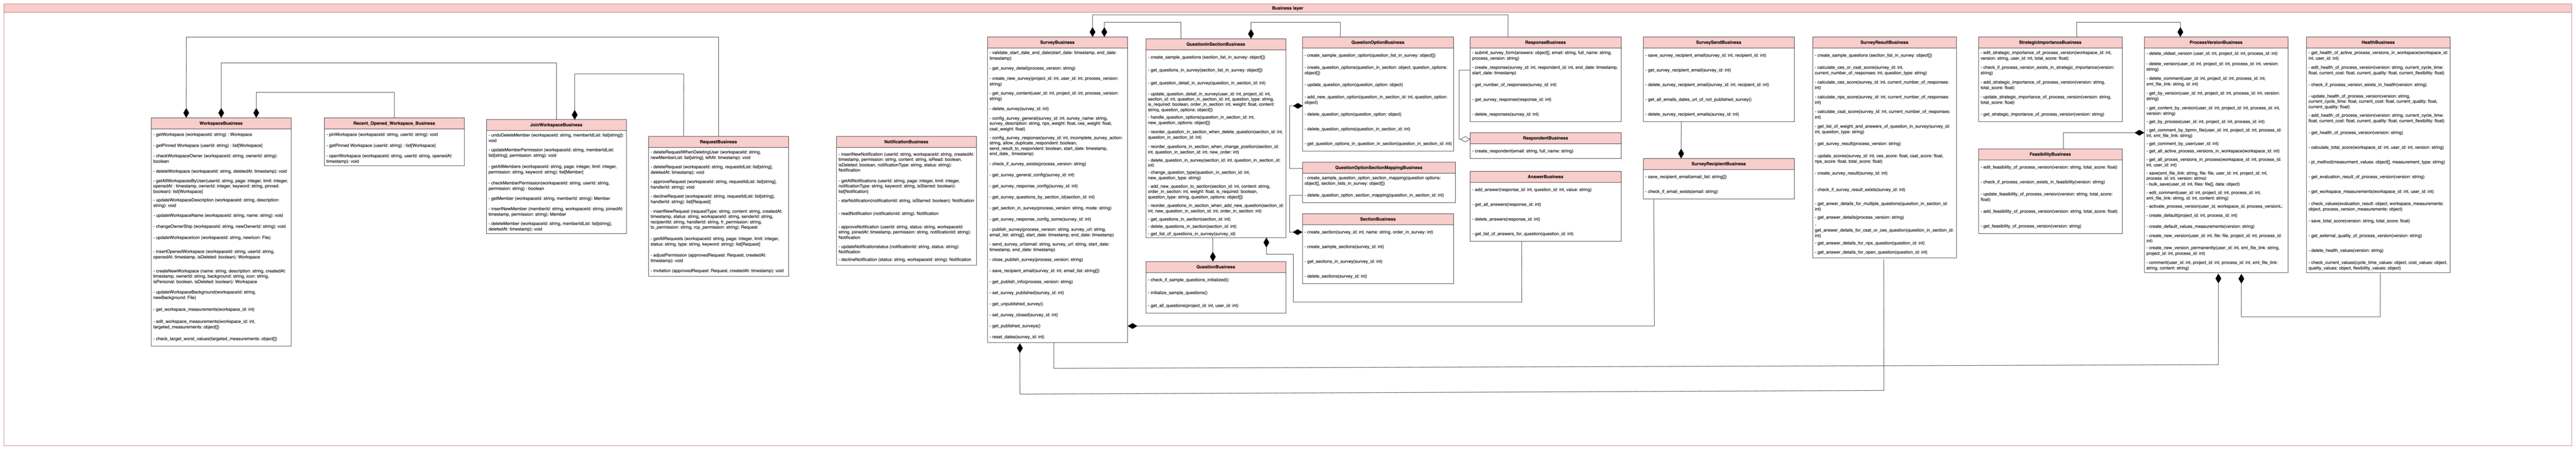
\includegraphics[ width = \linewidth]{Content/Phân tích và thiết kế hệ thống/documents/Sơ đồ lớp/images/Business layer/businessLayer2.png}
    \vspace{0.5cm}
    \caption{Tổng quan Business Layer}
    \label{fig:Tổng quan Business Layer}
\end{figure}

Nhiệm vụ của tầng Business là phân tích những yêu cầu được gửi từ tầng Presentation, xử lý logic nghiệp vụ và
gọi tới các đối tượng ở tầng Persistence để tương tác với cơ sở dữ liệu.

\begin{figure}[H]
    \centering
    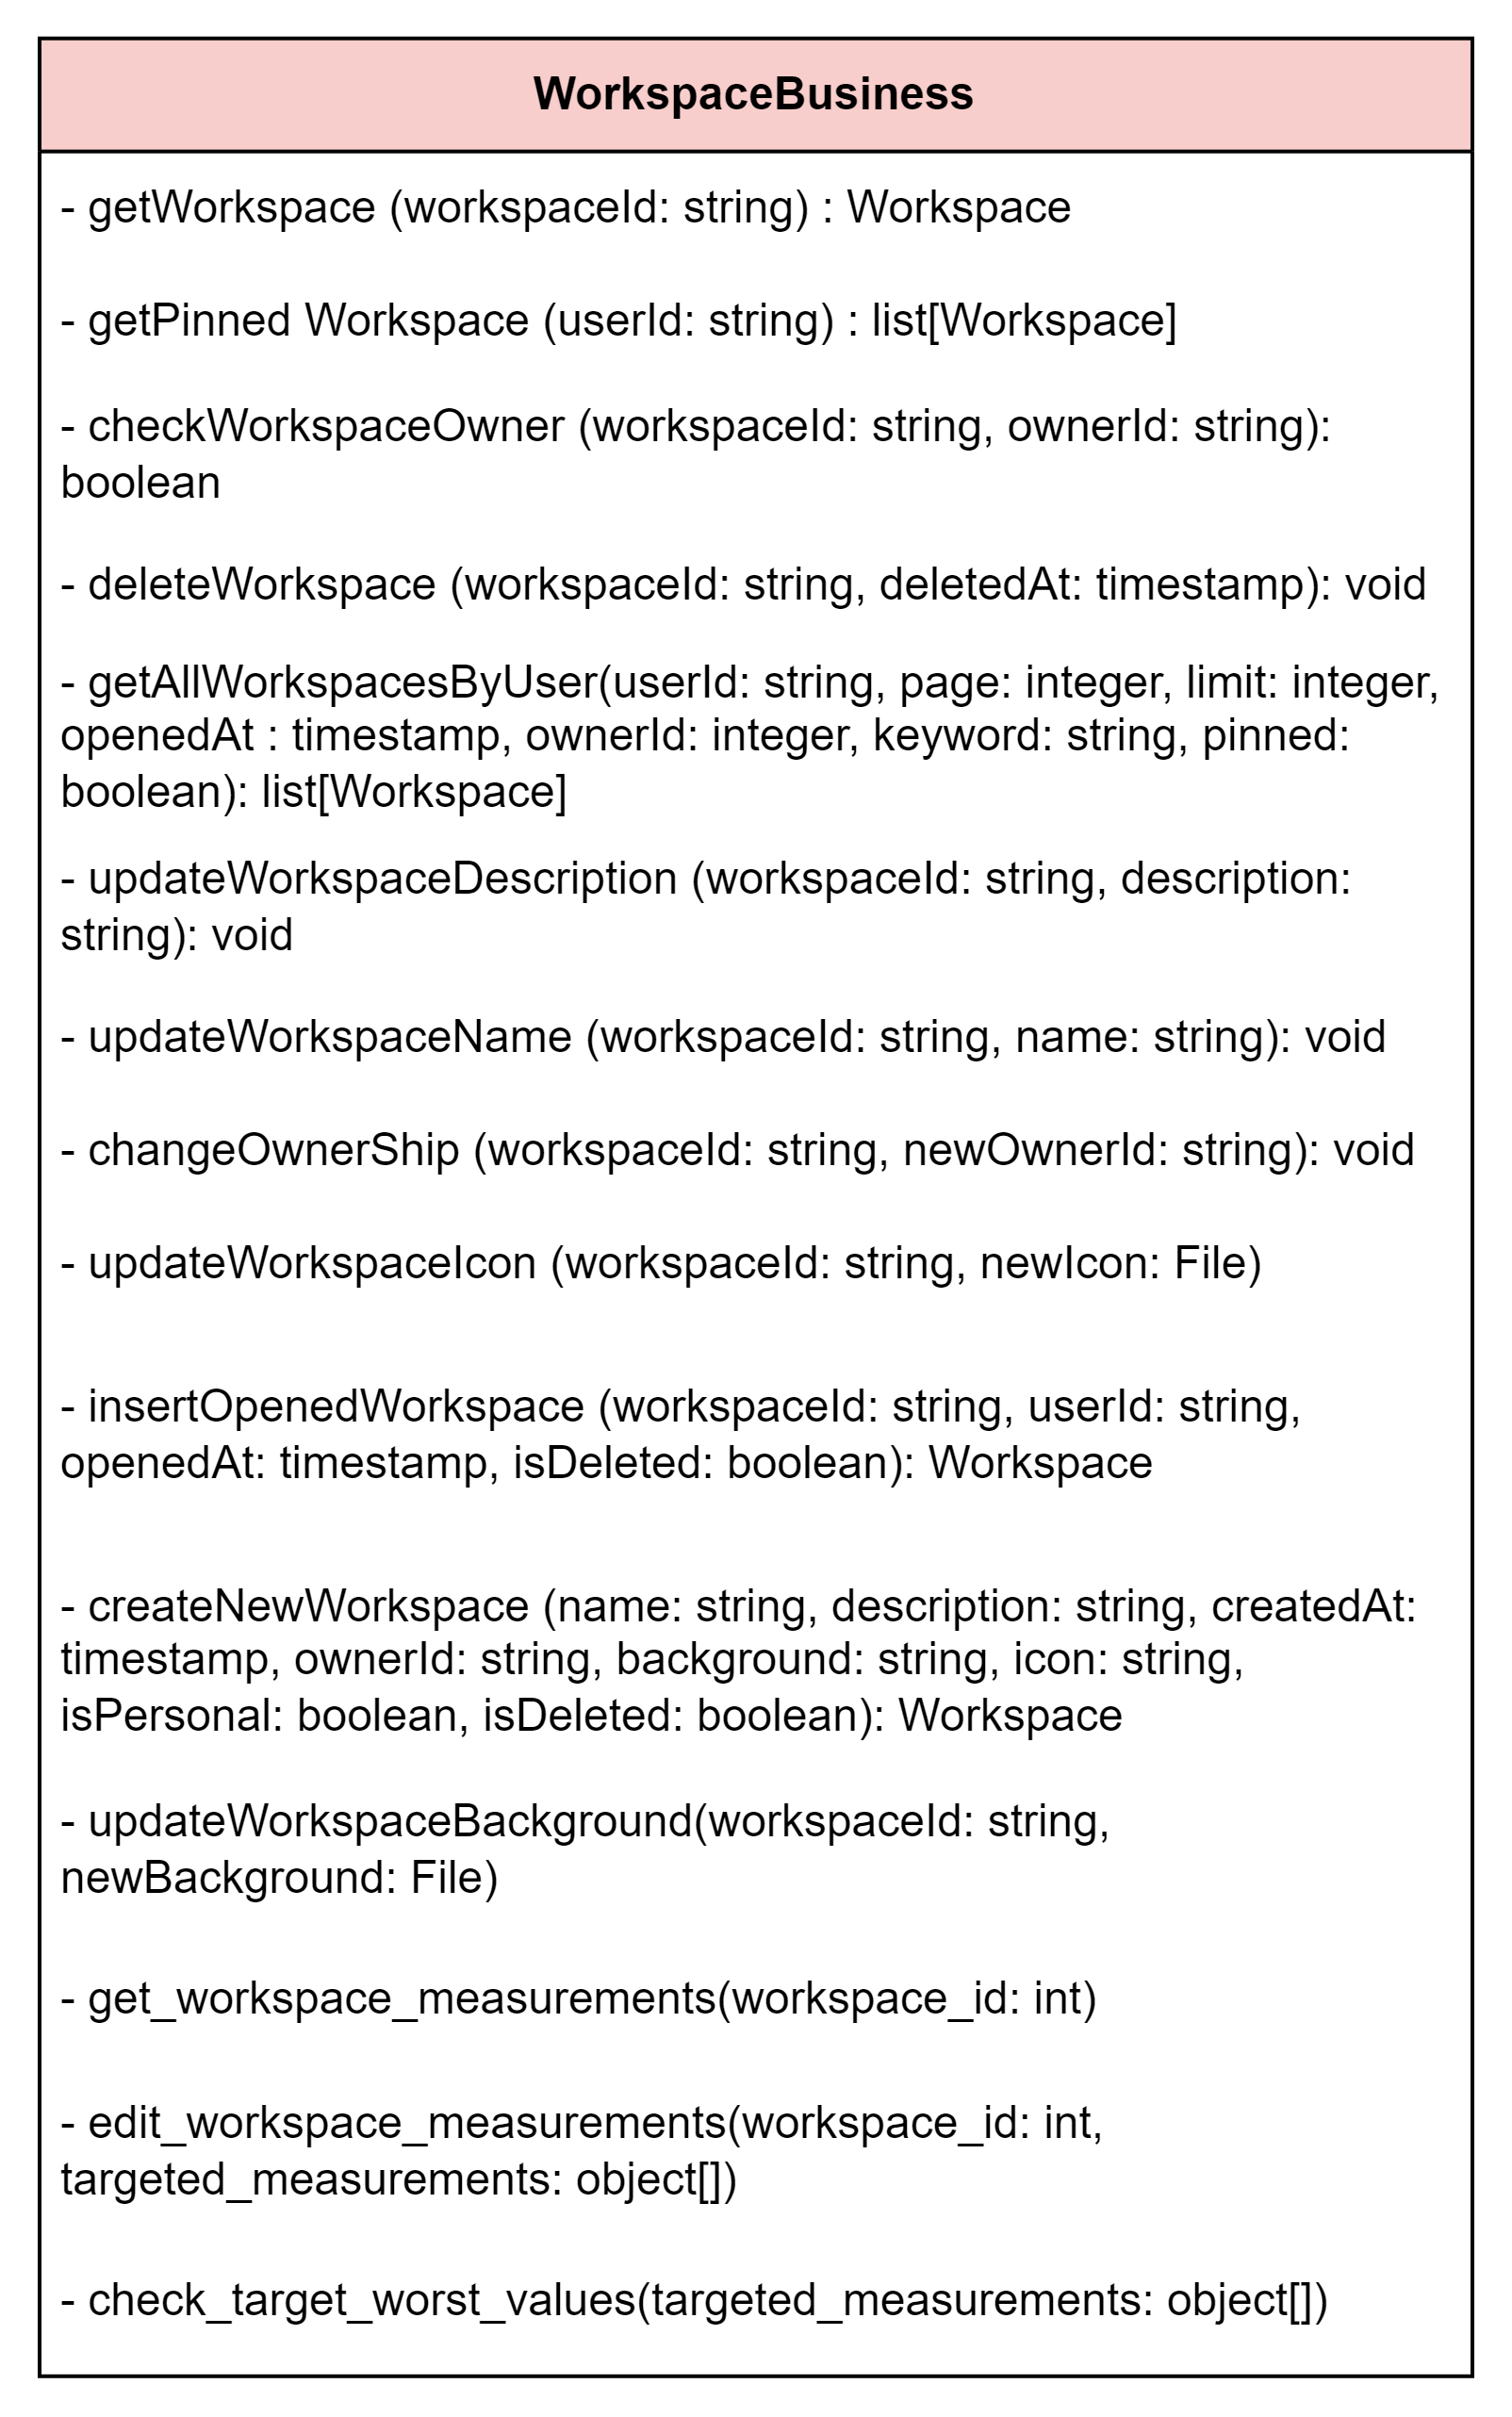
\includegraphics[ width = \linewidth]{Content/Phân tích và thiết kế hệ thống/documents/Sơ đồ lớp/images/Business layer/workspaceBusiness.png}
    \vspace{0.5cm}
    \caption{Class WorkspaceBusiness trong Business layer}
    \label{fig:Class WorkspaceBusiness trong Business layer}
\end{figure}

\par
Class WorkspaceBusiness là class chịu trách nhiệm xử lý logic nghiệp vụ liên quan
đến Workspace. Class này sẽ thừa kế các class khác như: Workspace\_Get\_Business,
Workspace\_Delete\_Business, Workspace\_Update\_Business, Workspace\_Insert\_Business.
Những class này sẽ thực hiện các chức năng tương ứng với tên của chúng, như vậy,
bằng cách này sẽ giúp cho việc quản lý code dễ dàng hơn, và khi có sự thay đổi
trong một chức năng nào đó thì việc thay đổi này sẽ không ảnh hưởng đến các chức
năng khác. Ngoài ra, class Workspace\_Insert\_Business còn thừa kế class
Recent\_Opened\_Workspace\_Insert\_Business để thực hiện chức năng thêm mới vào 
bảng Recent\_Opened\_Workspace.
\begin{figure}[H]
    \centering
    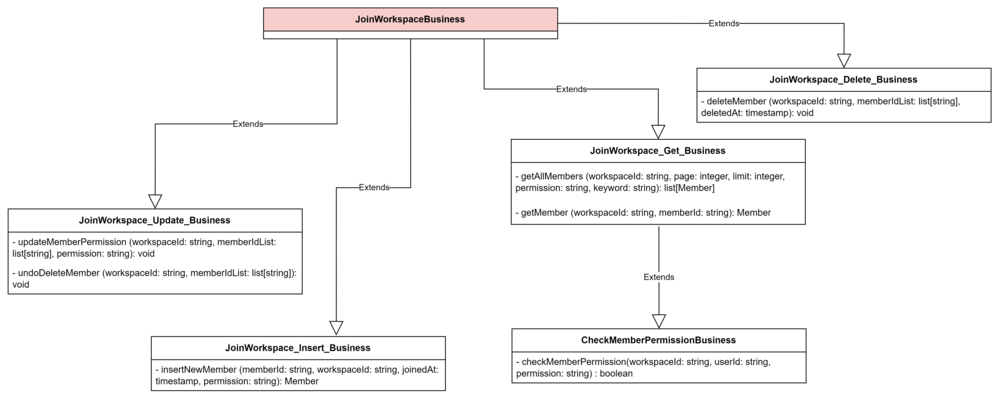
\includegraphics[ width = \linewidth]{Content/Phân tích và thiết kế hệ thống/documents/Sơ đồ lớp/images/Business layer/joinWorkspaceBusiness.png}
    \vspace{0.5cm}
    \caption{Class JoinWorkspaceBusiness trong Business layer}
    \label{fig:Class JoinWorkspaceBusiness trong Business layer}
\end{figure}
\par
Class Join\_Workspace\_Business là class chịu trách nhiệm xử lý logic nghiệp vụ liên quan đến
việc người dùng tham gia vào một Workspace. Class này sẽ thừa kế các class khác như:
Join\_Workspace\_Get\_Business, Join\_Workspace\_Delete\_Business, Join\_Workspace\_Update\_Business.
Những class này sẽ thực hiện các chức năng tương ứng với tên của chúng. Ngoài ra, class
JoinWorkspace\_Get\_Business còn kế thừa từ class CheckMemberPermissionBusiness để thực hiện
chức năng kiểm tra quyền của người dùng trong một Workspace.
\begin{figure}[H]
    \centering
    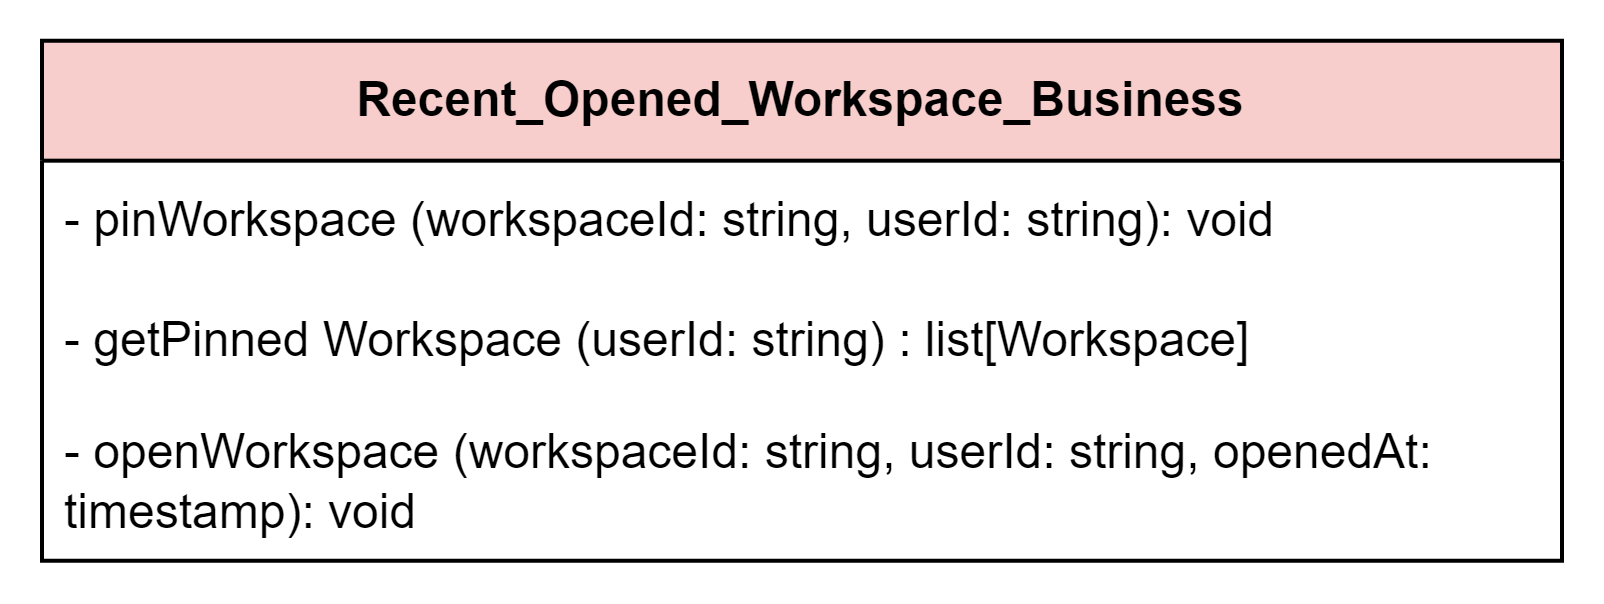
\includegraphics[ width = \linewidth]{Content/Phân tích và thiết kế hệ thống/documents/Sơ đồ lớp/images/Business layer/recentOpenedWorkspaceBusiness.png}
    \vspace{0.5cm}
    \caption{Class RecentOpenedWorkspaceBusiness trong Business layer}
    \label{fig:Class RecentOpenedWorkspaceBusiness trong Business layer}
\end{figure}
\par
Class Recent\_Opened\_Workspace\_Business là class chịu trách nhiệm xử lý logic
cho nghiệp vụ liên quan đến những workspace được mở gần đây của người dùng.
Class này chỉ kế thừa hai class khác: Recent\_Opened\_Workspace\_Get\_Business và
Recent\_Opened\_Workspace\_Update\_Business cho những xử lý logic khi lấy danh sách 
Workspace được đánh dấu và logic mở cũng như đánh dấu một Workspace.
\begin{figure}[H]
    \centering
    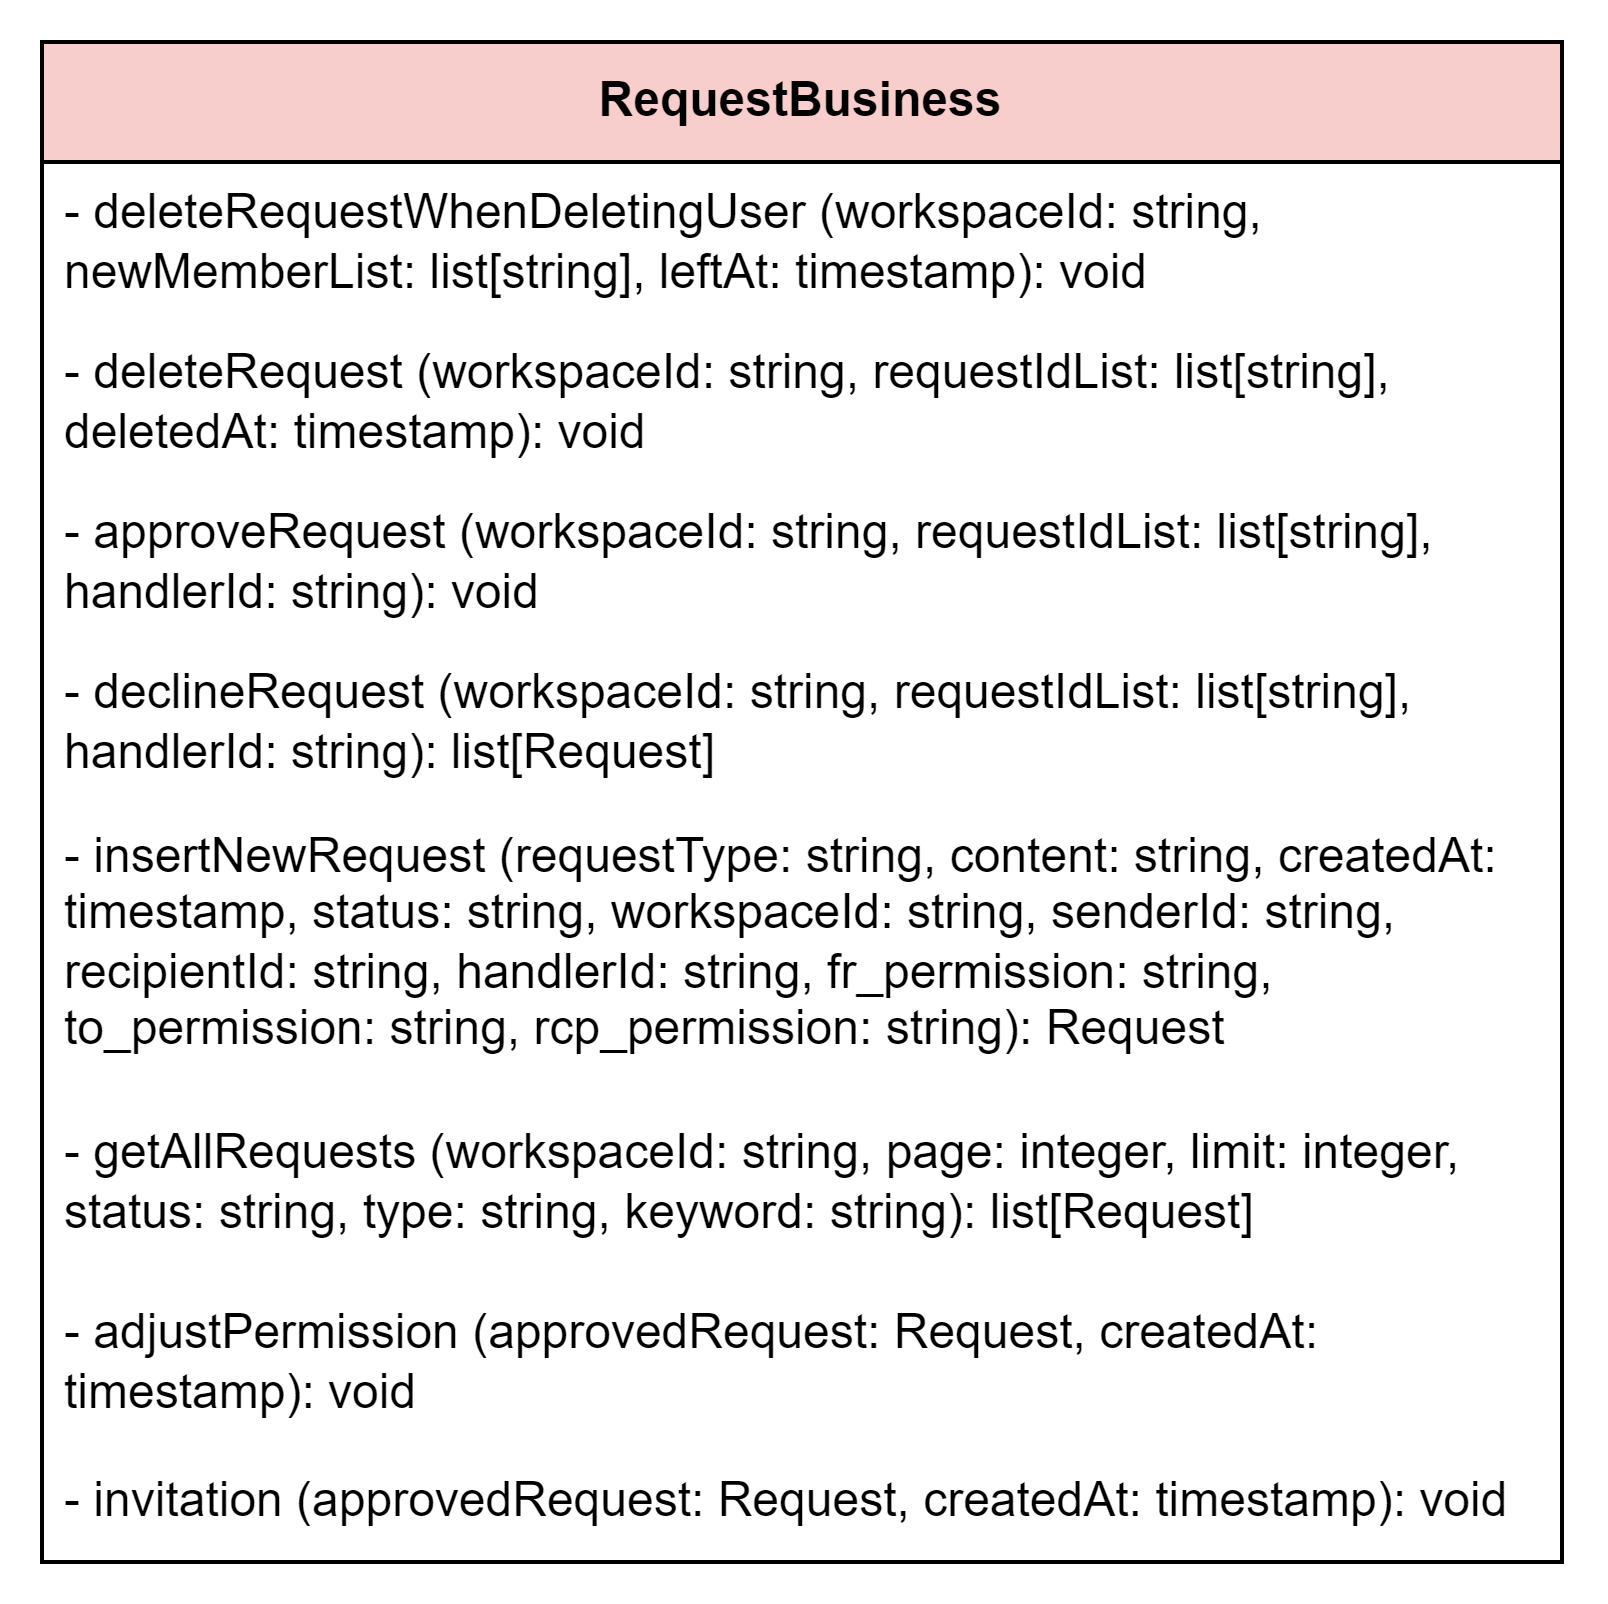
\includegraphics[ width = \linewidth]{Content/Phân tích và thiết kế hệ thống/documents/Sơ đồ lớp/images/Business layer/requestBusiness.png}
    \vspace{0.5cm}
    \caption{Class RequestBusiness trong Business layer}
    \label{fig:Class RequestBusiness trong Business layer}
\end{figure}
\par
Class RequestBusiness là class chịu trách nhiệm xử lý logic nghiệp vụ liên quan đến
những yêu cầu trong một Workspace. Class này sẽ thừa kế các class khác như:
Request\_Get\_Business, Request\_Delete\_Business, Request\_Update\_Business, Request\_Insert\_Business.
Những class này sẽ thực hiện các chức năng tương ứng với tên của chúng. Ngoài ra, class
Request\_Update\_Business còn kế thừa từ class Request\_Handling\_Business, class này sẽ thực
hiện chức năng xử lý những yêu cầu.
\begin{figure}[H]
    \centering
    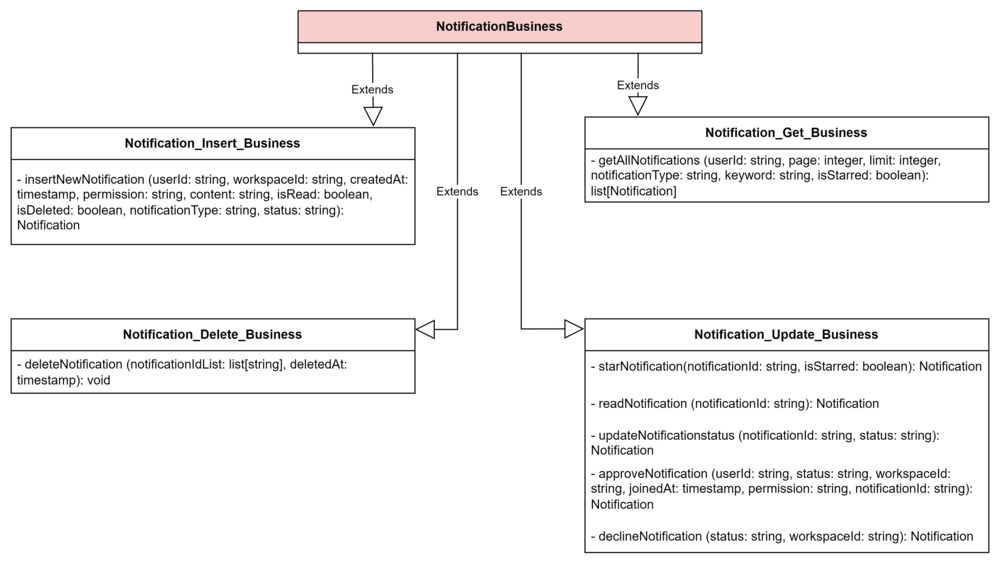
\includegraphics[ width = \linewidth]{Content/Phân tích và thiết kế hệ thống/documents/Sơ đồ lớp/images/Business layer/notificationBusiness.png}
    \vspace{0.5cm}
    \caption{Class NotificationBusiness trong Business layer}
    \label{fig:Class NotificationBusiness trong Business layer}
\end{figure}
\par
Class NotificationBusiness là class chịu trách nhiệm xử lý logic nghiệp vụ liên quan đến
những thông báo trong một Workspace. Tương tự như những class trên, class này sẽ thừa kế các class khác như:
Notification\_Get\_Business, Notification\_Delete\_Business, Notification\_Update\_Business, Notification\_Insert\_Busines.

%% SURVEY %%
\begin{figure}[H]
    \centering
    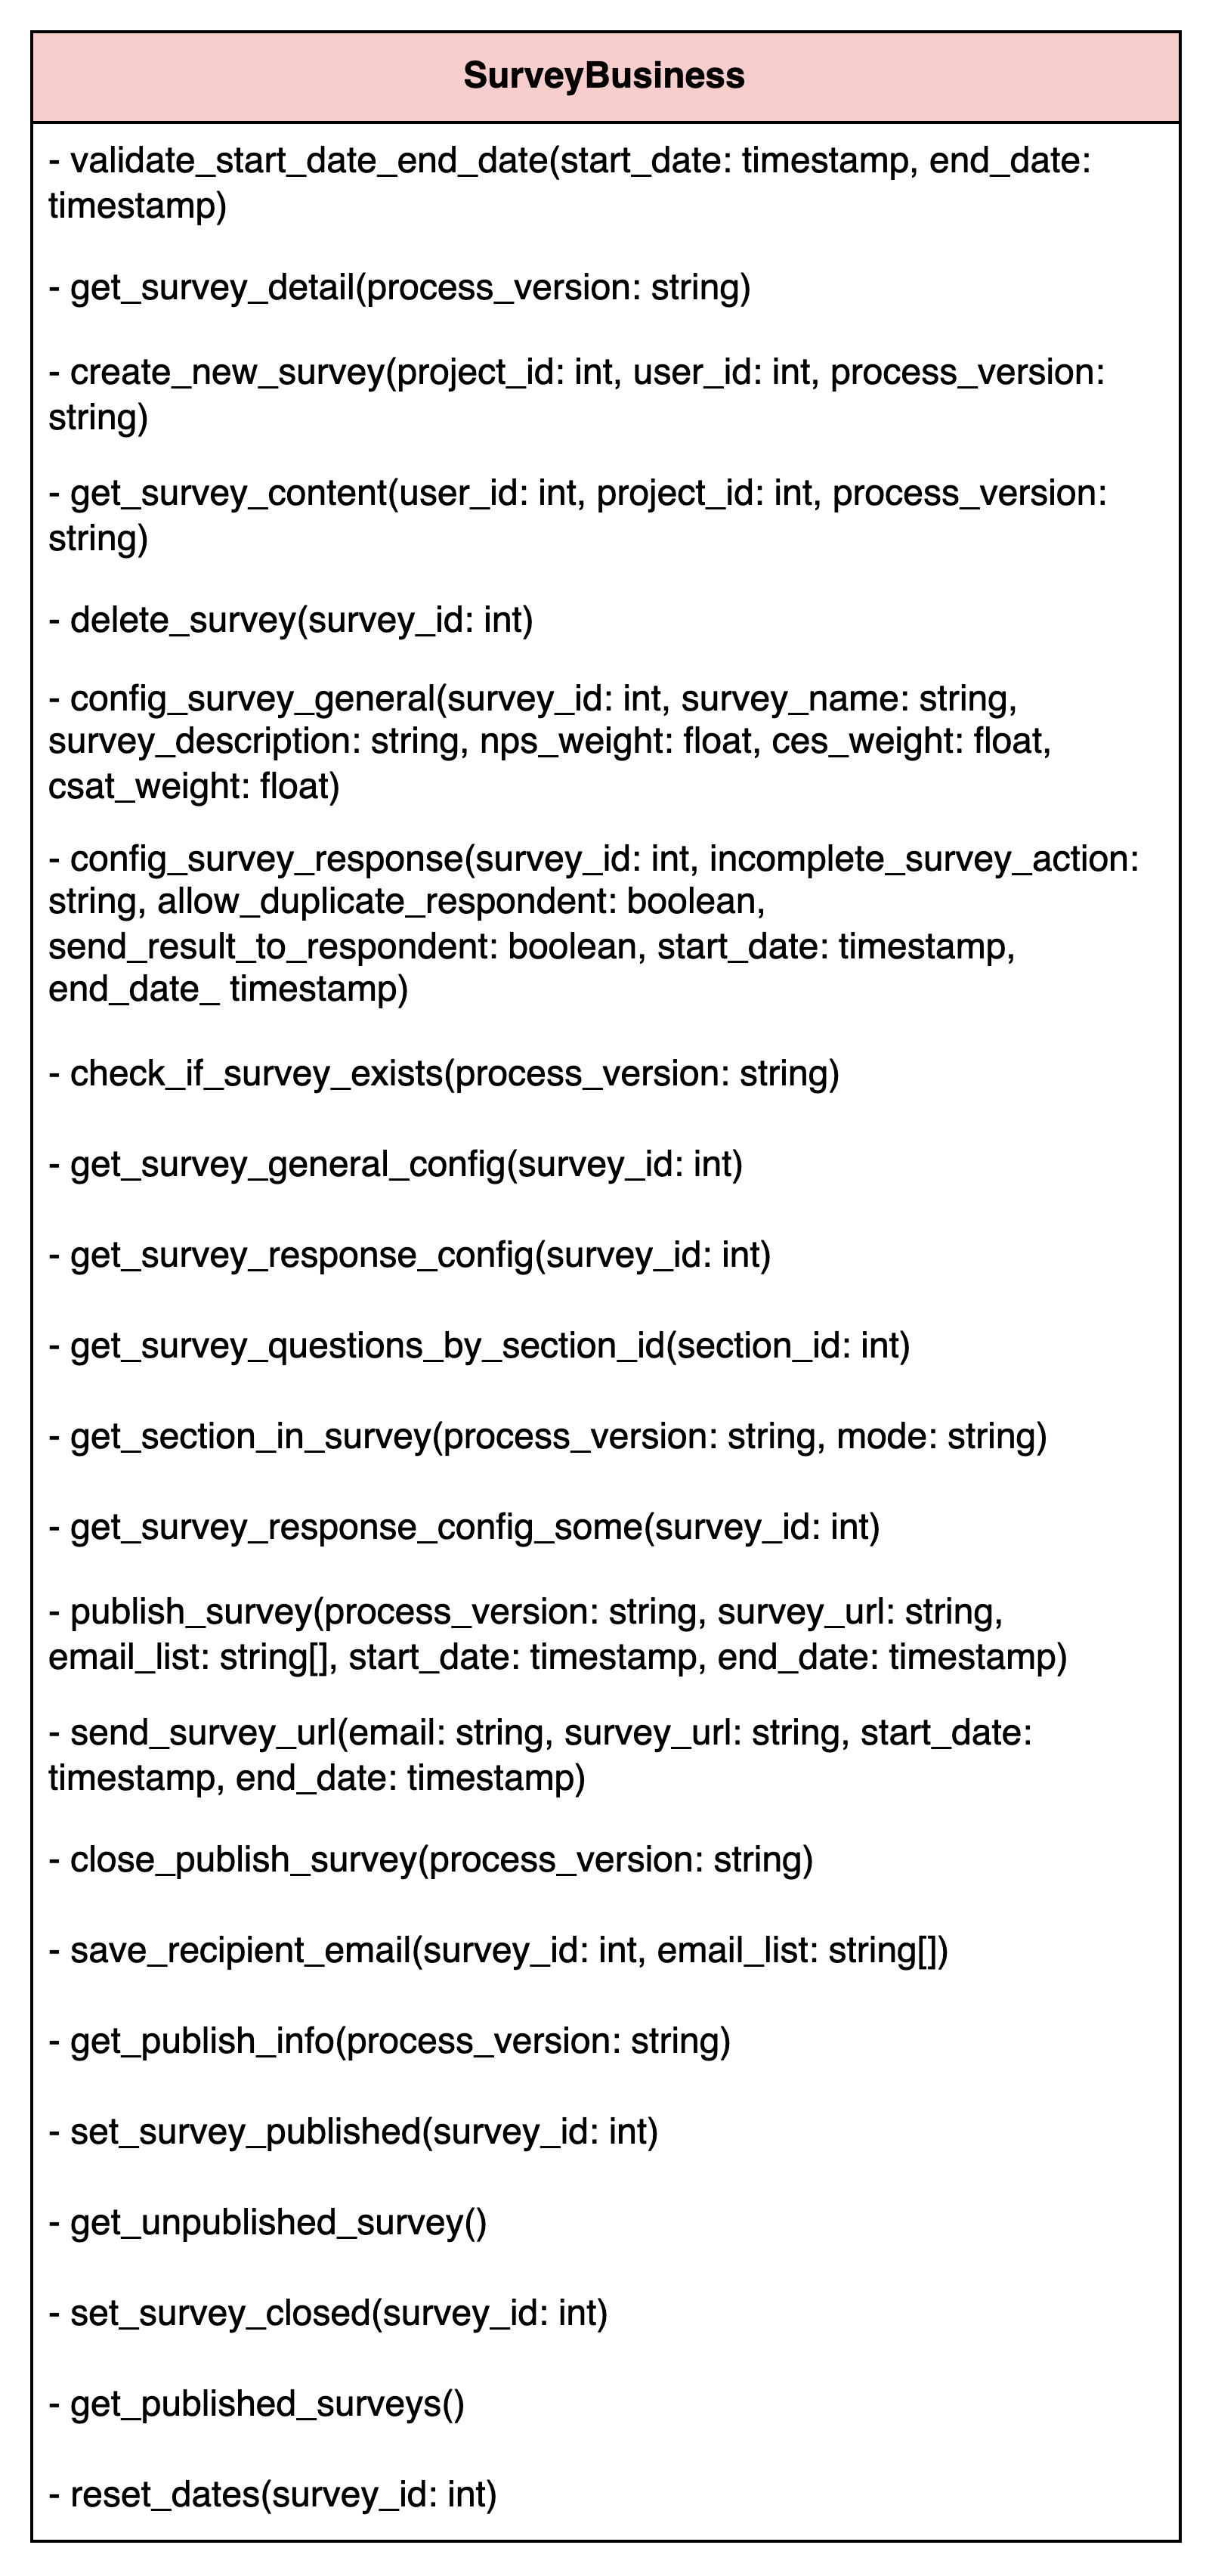
\includegraphics[ width = 0.5\linewidth]{Content/Phân tích và thiết kế hệ thống/documents/Sơ đồ lớp/images/Business layer/survey.png}
    \vspace{0.5cm}
    \caption{Class SurveyBusiness trong Business layer}
    \label{fig:Class SurveyBusiness trong Business layer}
\end{figure}
\par
Class SurveyBusiness chịu trách nhiệm xử lý các logic liên quan đến bảng khảo sát. Một số phương thức xử lý chẳng hạn như, 
lấy toàn bộ nội dung của bảng khảo sát, gửi email đường dẫn bảng khảo sát tới một số người dùng, công bố bảng khảo sát, chỉnh sửa những thiết lập liên quan đến bảng khảo sát.
\begin{figure}[H]
    \centering
    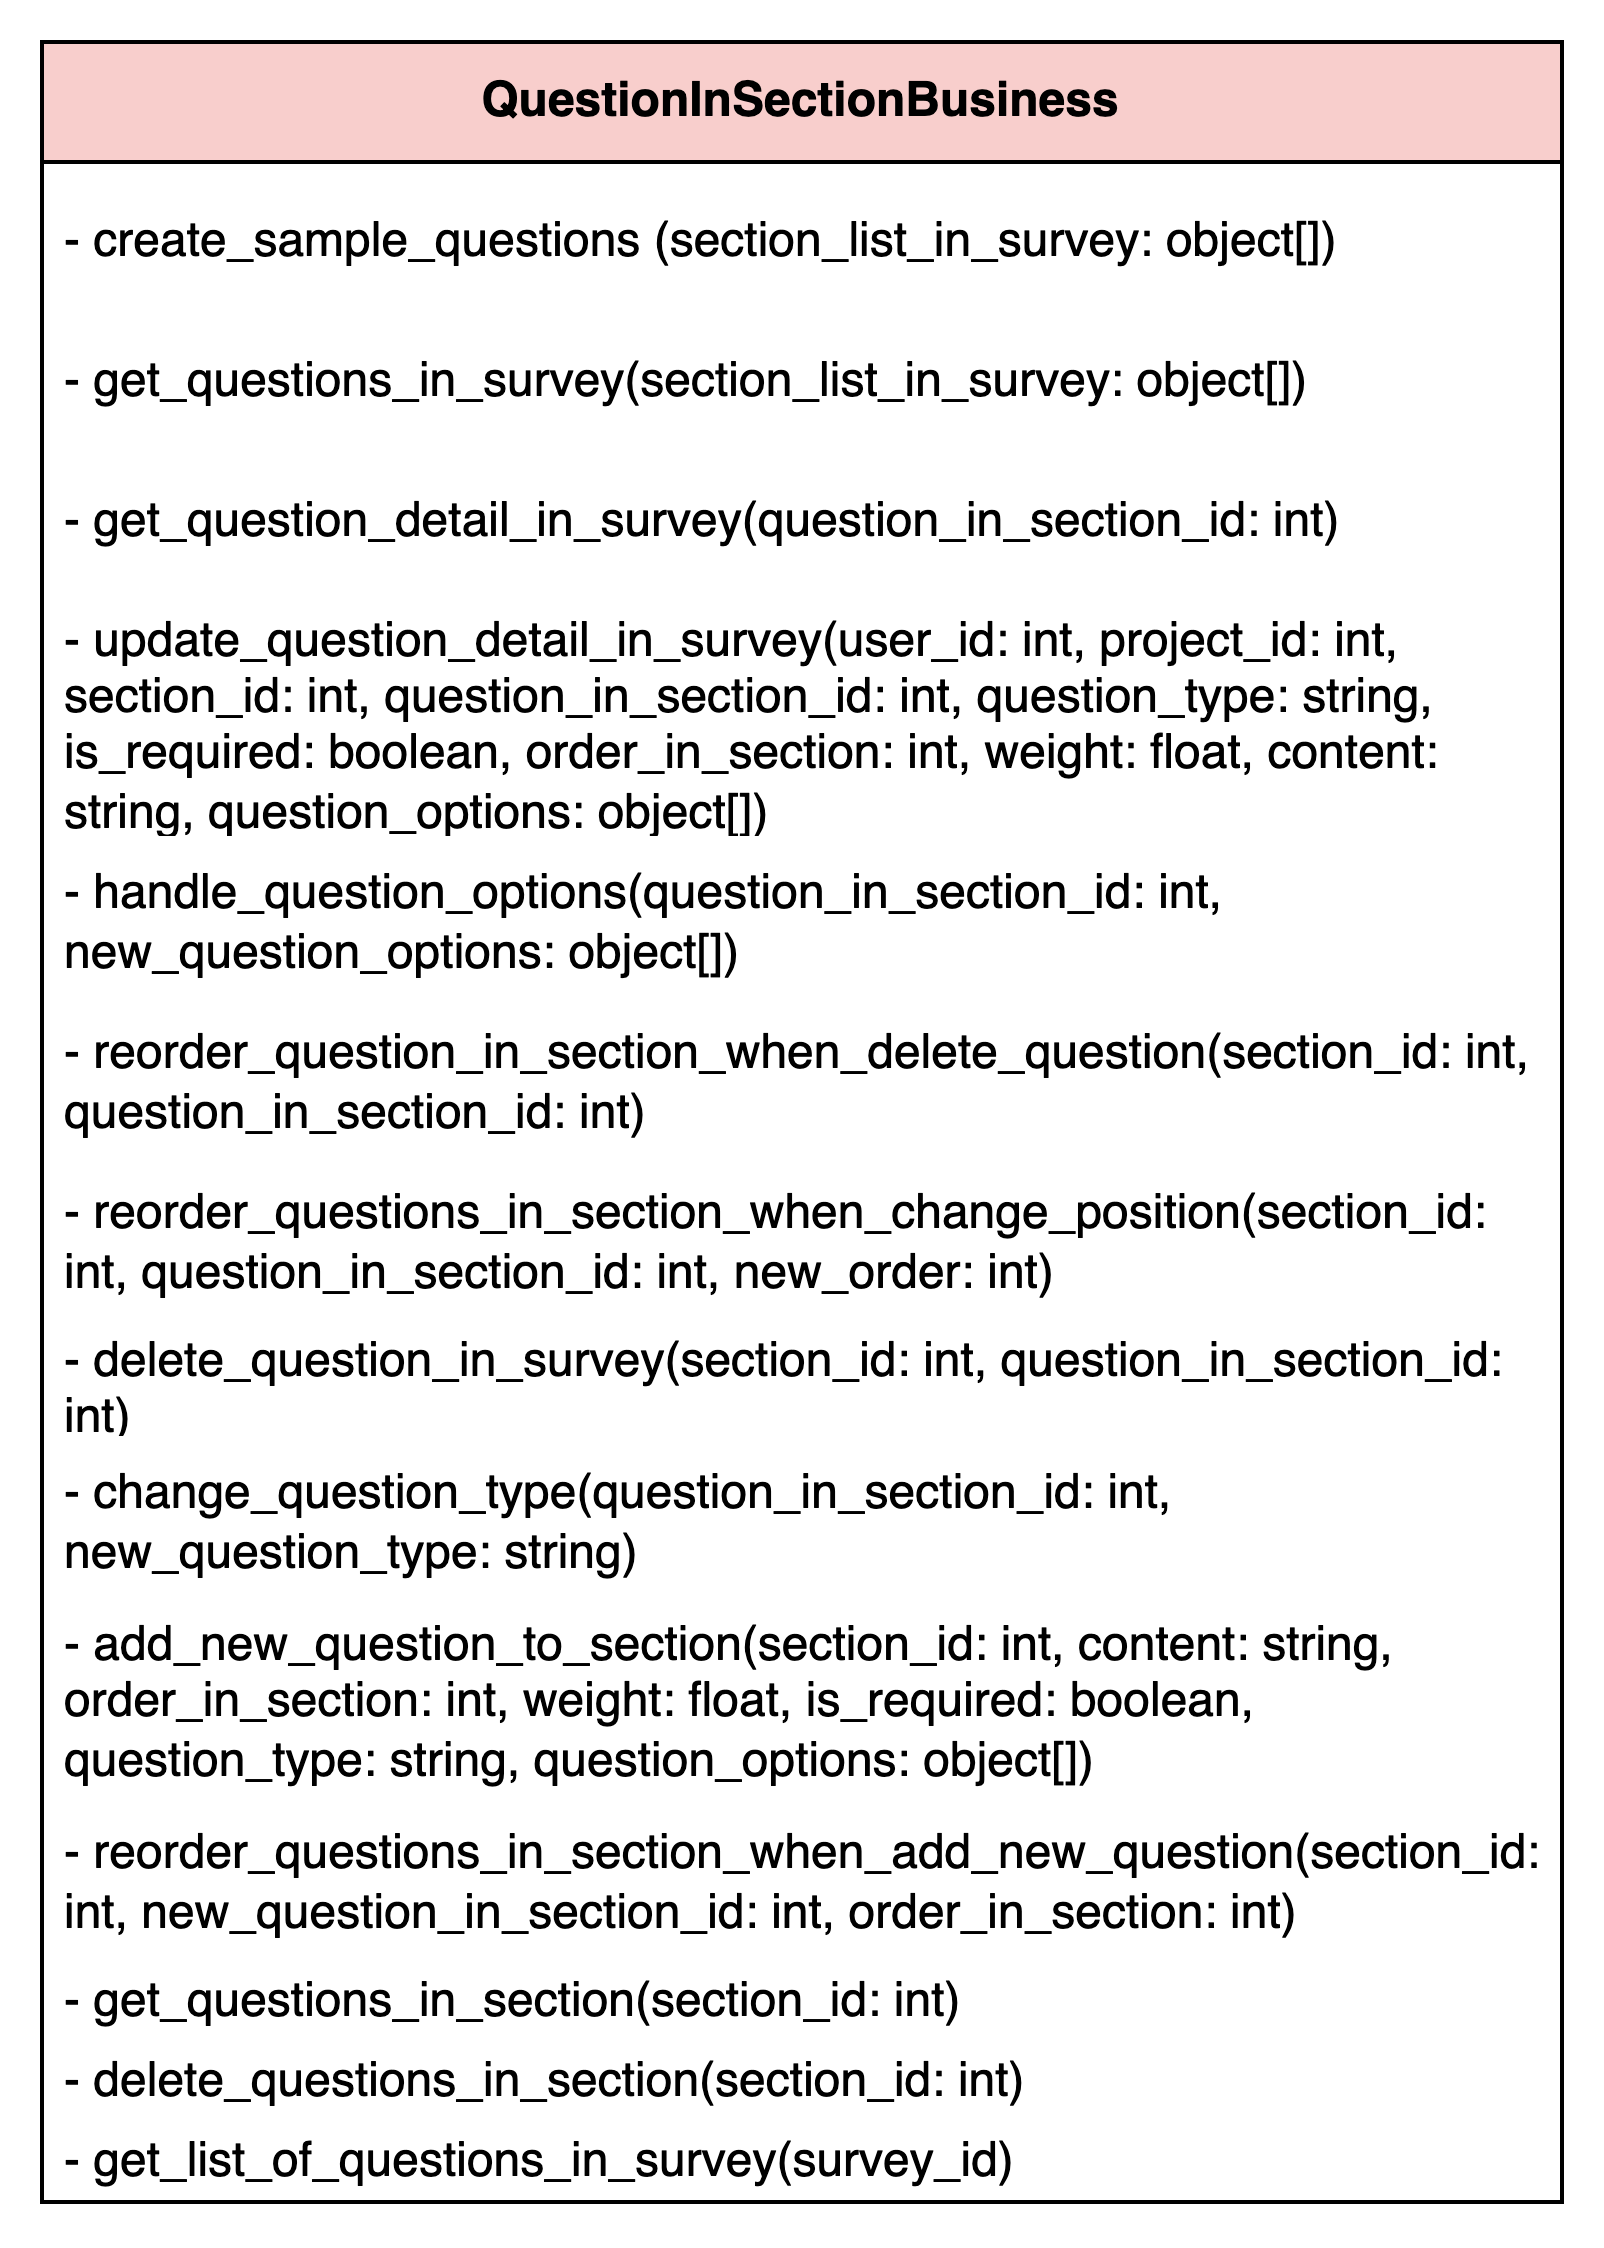
\includegraphics[ width = 0.5\linewidth]{Content/Phân tích và thiết kế hệ thống/documents/Sơ đồ lớp/images/Business layer/questionInSection.png}
    \vspace{0.5cm}
    \caption{Class QuestionInSectionBusiness trong Business layer}
    \label{fig:Class QuestionInSectionBusiness trong Business layer}
\end{figure}
\par
Class QuestionInSectionBusiness sẽ xử lý những logic liên quan đến các câu hỏi có trong bảng khảo sát, chẳng hạn như lấy nội dung của câu hỏi, 
xóa câu hỏi được chọn và sắp xếp thứ tự những câu hỏi còn lại, thêm câu hỏi mới, thay đổi nội dung, thiết lập của câu hỏi.
\begin{figure}[H]
    \centering
    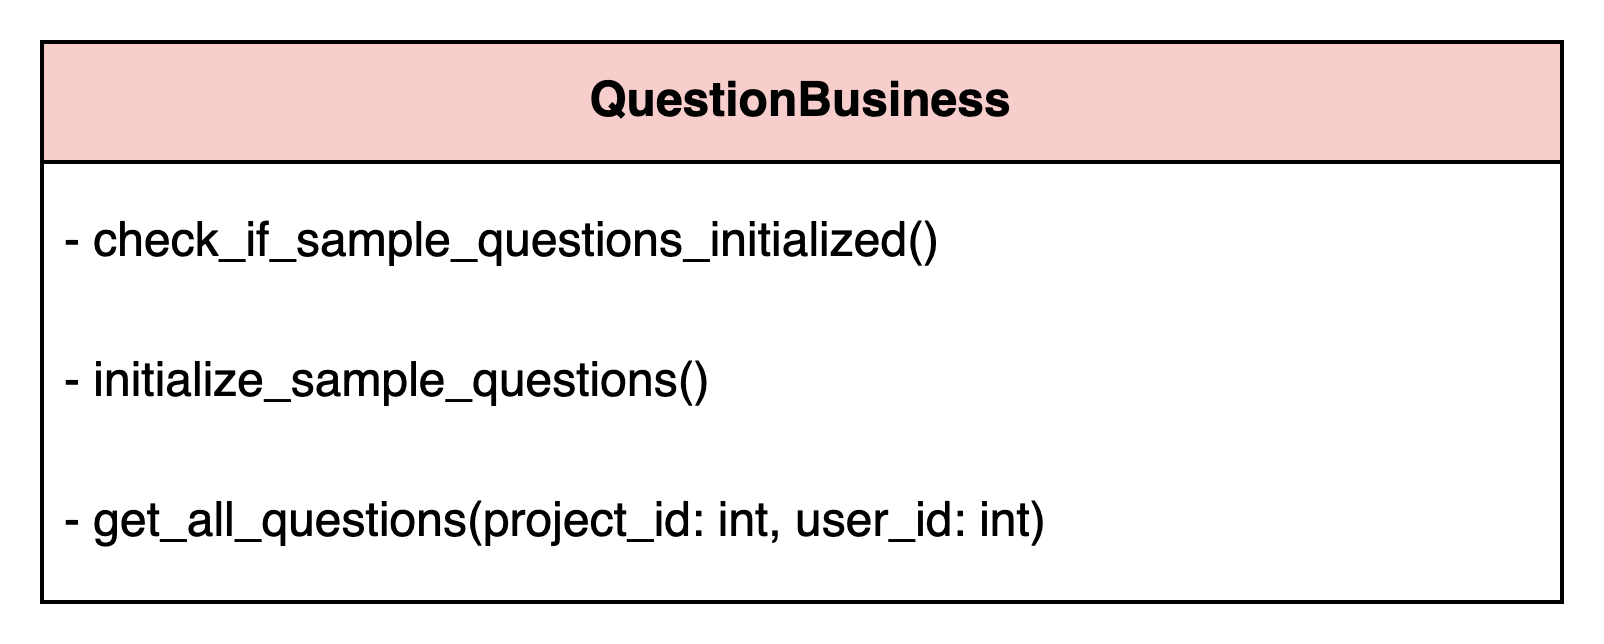
\includegraphics[ width = 0.5\linewidth]{Content/Phân tích và thiết kế hệ thống/documents/Sơ đồ lớp/images/Business layer/question.png}
    \vspace{0.5cm}
    \caption{Class QuestionBusiness trong Business layer}
    \label{fig:Class QuestionBusiness trong Business layer}
\end{figure}
\par
Class QuestionBusiness xử lý những logic liên quan đến những câu hỏi có sẵn trong hệ thống. Khi survey được khởi tạo, các câu hỏi mẫu có sẵn 
trong survey sẽ được lấy từ câu hỏi đã có trong hệ thống. Một số phương thức xử lý như khởi tạo câu hỏi mẫu, lấy toàn bộ các câu hỏi, hay kiểm tra xem câu hỏi đã được khởi tạo hay chưa.
\begin{figure}[H]
    \centering
    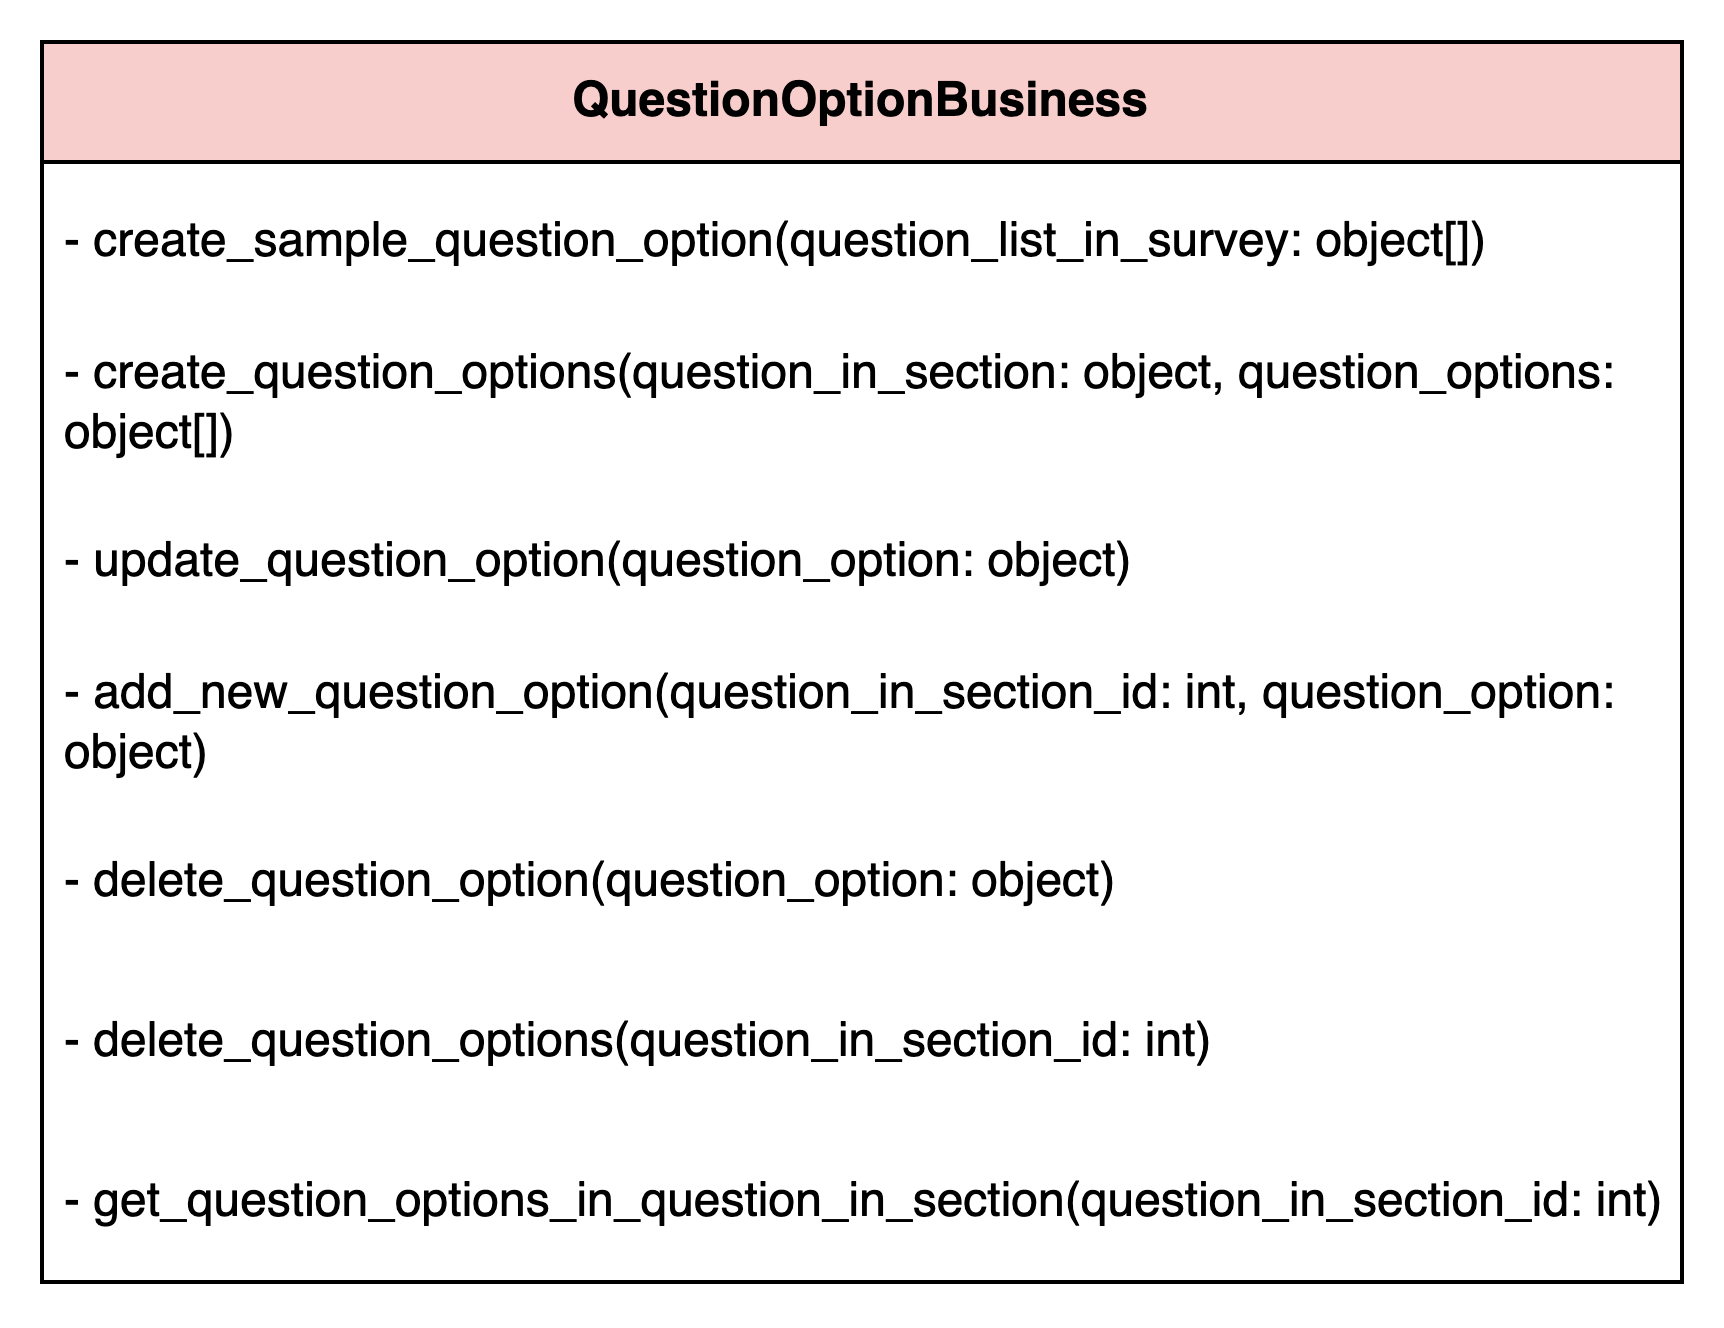
\includegraphics[ width = 0.5\linewidth]{Content/Phân tích và thiết kế hệ thống/documents/Sơ đồ lớp/images/Business layer/questionOption.png}
    \vspace{0.5cm}
    \caption{Class QuestionOptionBusiness trong Business layer}
    \label{fig:Class QuestionOptionBusiness trong Business layer}
\end{figure}
\par
Class QuestionOptionBusiness sẽ xử lý những logic liên quan đến các lựa chọn trong mỗi câu hỏi, ứng với các câu hỏi dạng multiple choice. 
Một số phương thức xử lý như: khởi tạo các lựa chọn, thêm, sửa, xóa các lựa chọn, thay đổi thứ tự các lựa chọn khi người dùng kéo thả.
\begin{figure}[H]
    \centering
    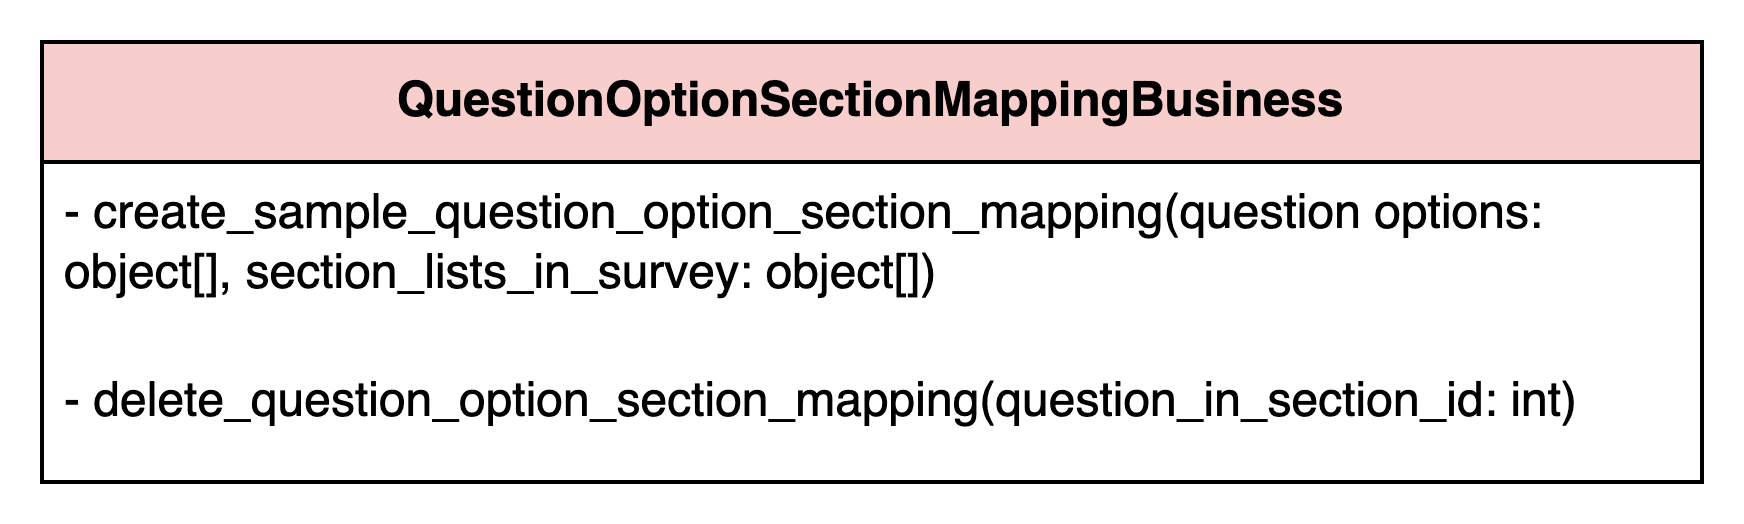
\includegraphics[ width = 0.5\linewidth]{Content/Phân tích và thiết kế hệ thống/documents/Sơ đồ lớp/images/Business layer/questionOptionSectionMapping.png}
    \vspace{0.5cm}
    \caption{Class QuestionOptionSectionMappingBusiness trong Business layer}
    \label{fig:Class QuestionOptionSectionMappingBusiness trong Business layer}
\end{figure}
\par
Class QuestionOptionSectionMappingBusiness sẽ tập trung xử lý những logic liên quan tới việc khi người dùng chọn các đáp án khác nhau sẽ được 
điều hướng tới những phần khác nhau trong bảng khảo sát. Ở đây có một số phương thức xử lý như khởi tạo việc tham chiếu lựa chọn này tới một phần nào đó 
trong bảng khảo sát, hay xóa đi mối quan hệ tham chiếu đó.
\begin{figure}[H]
    \centering
    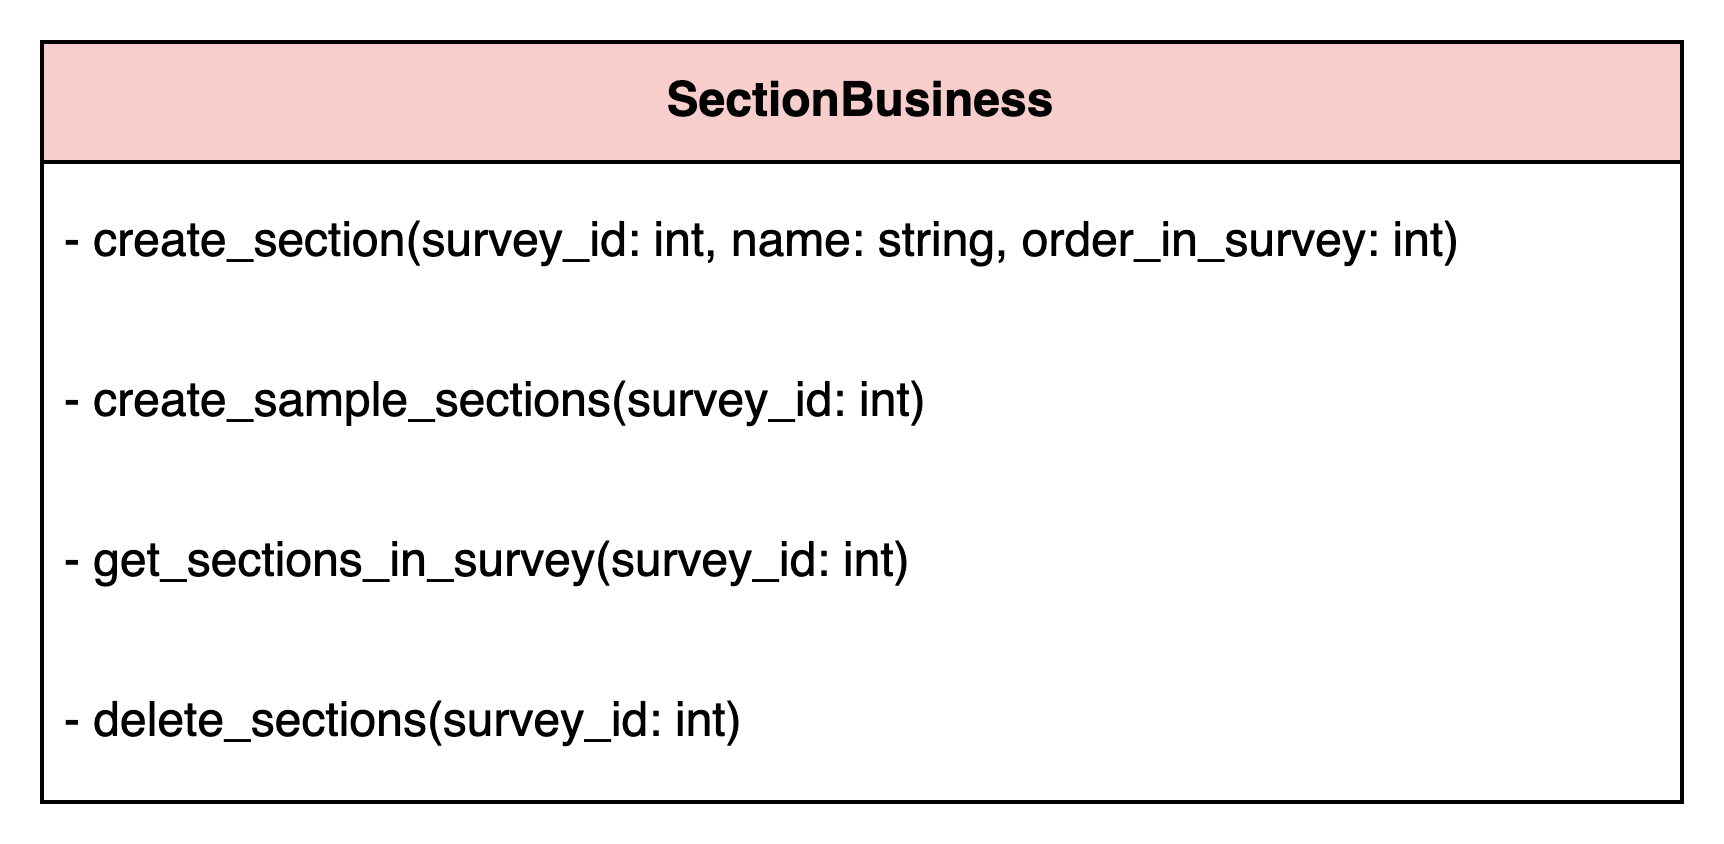
\includegraphics[ width = 0.5\linewidth]{Content/Phân tích và thiết kế hệ thống/documents/Sơ đồ lớp/images/Business layer/section.png}
    \vspace{0.5cm}
    \caption{Class SectionBusiness trong Business layer}
    \label{fig:Class SectionBusiness trong Business layer}
\end{figure}
\par
Class SectionBusiness sẽ quản lý việc xử lý logic đối với các phần trong bảng khảo sát. Bảng khảo sát được chia thành nhiều phần khác nhau để phân loại 
các nhóm câu hỏi, hướng tới những nhóm người dùng khác nhau cần được khảo sát. Các phương thức xử lý chẳng hạn như lấy các phần trong bảng khảo sát, xóa phần hay tạo mới phần.
\begin{figure}[H]
    \centering
    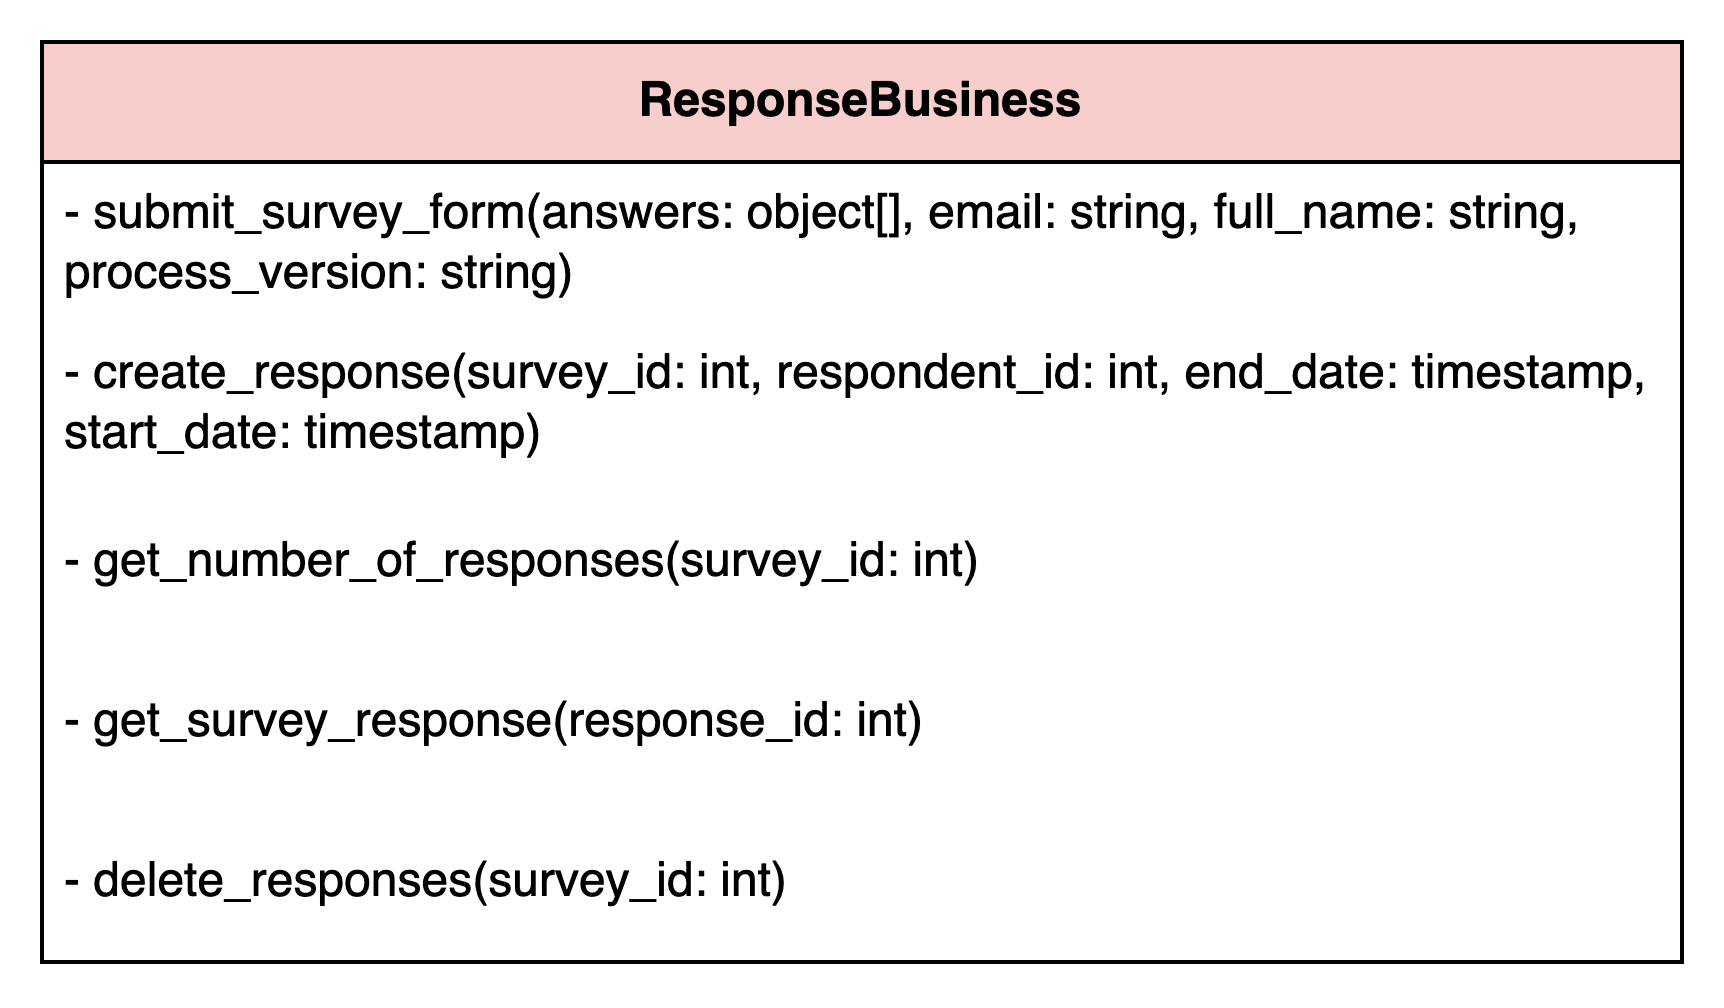
\includegraphics[ width = 0.5\linewidth]{Content/Phân tích và thiết kế hệ thống/documents/Sơ đồ lớp/images/Business layer/response.png}
    \vspace{0.5cm}
    \caption{Class ResponseBusiness trong Business layer}
    \label{fig:Class ResponseBusiness trong Business layer}
\end{figure}
\par
Class ResponseBusiness phụ trách những logic liên quan đến việc người dùng thực hiện và gửi bài làm khảo sát về cho hệ thống. 
Một số hàm xử lý logic chẳng hạn như làm và nộp bài làm khảo sát, lấy số lượng các bài làm hiện có của bài khảo sát,...
\begin{figure}[H]
    \centering
    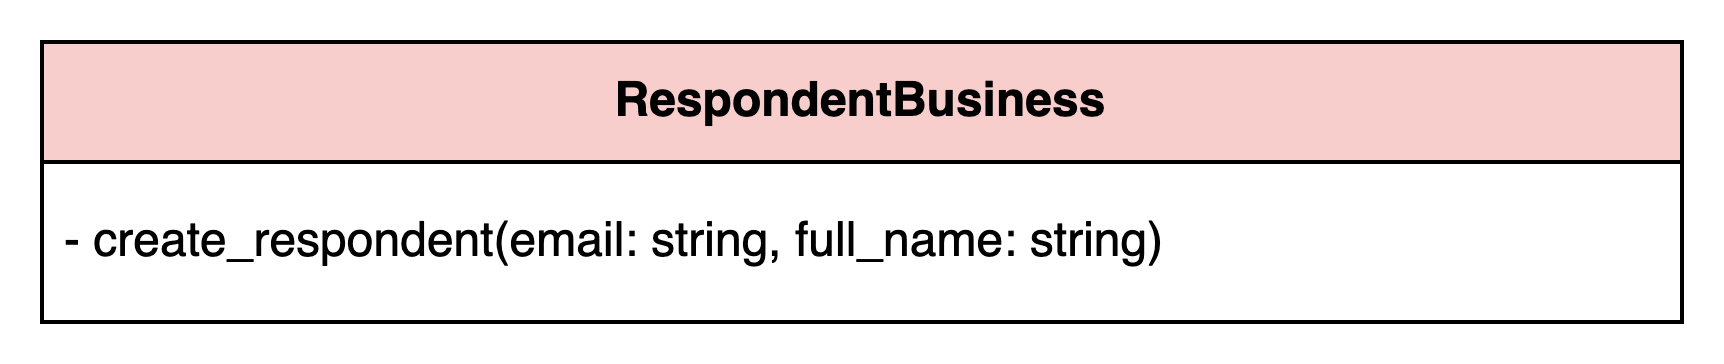
\includegraphics[ width = 0.5\linewidth]{Content/Phân tích và thiết kế hệ thống/documents/Sơ đồ lớp/images/Business layer/respondent.png}
    \vspace{0.5cm}
    \caption{Class RespondentBusiness trong Business layer}
    \label{fig:Class RespondentBusiness trong Business layer}
\end{figure}
\par
Class RespondentBusiness bao gồm logic cho việc tạo ra dữ liệu của người dùng tham gia làm bài khảo sát. Class này có một phương thức xử lý là khởi 
tạo dữ liệu của người dùng, bao gồm 2 tham số là email và tên đầy đủ của người dùng.
\begin{figure}[H]
    \centering
    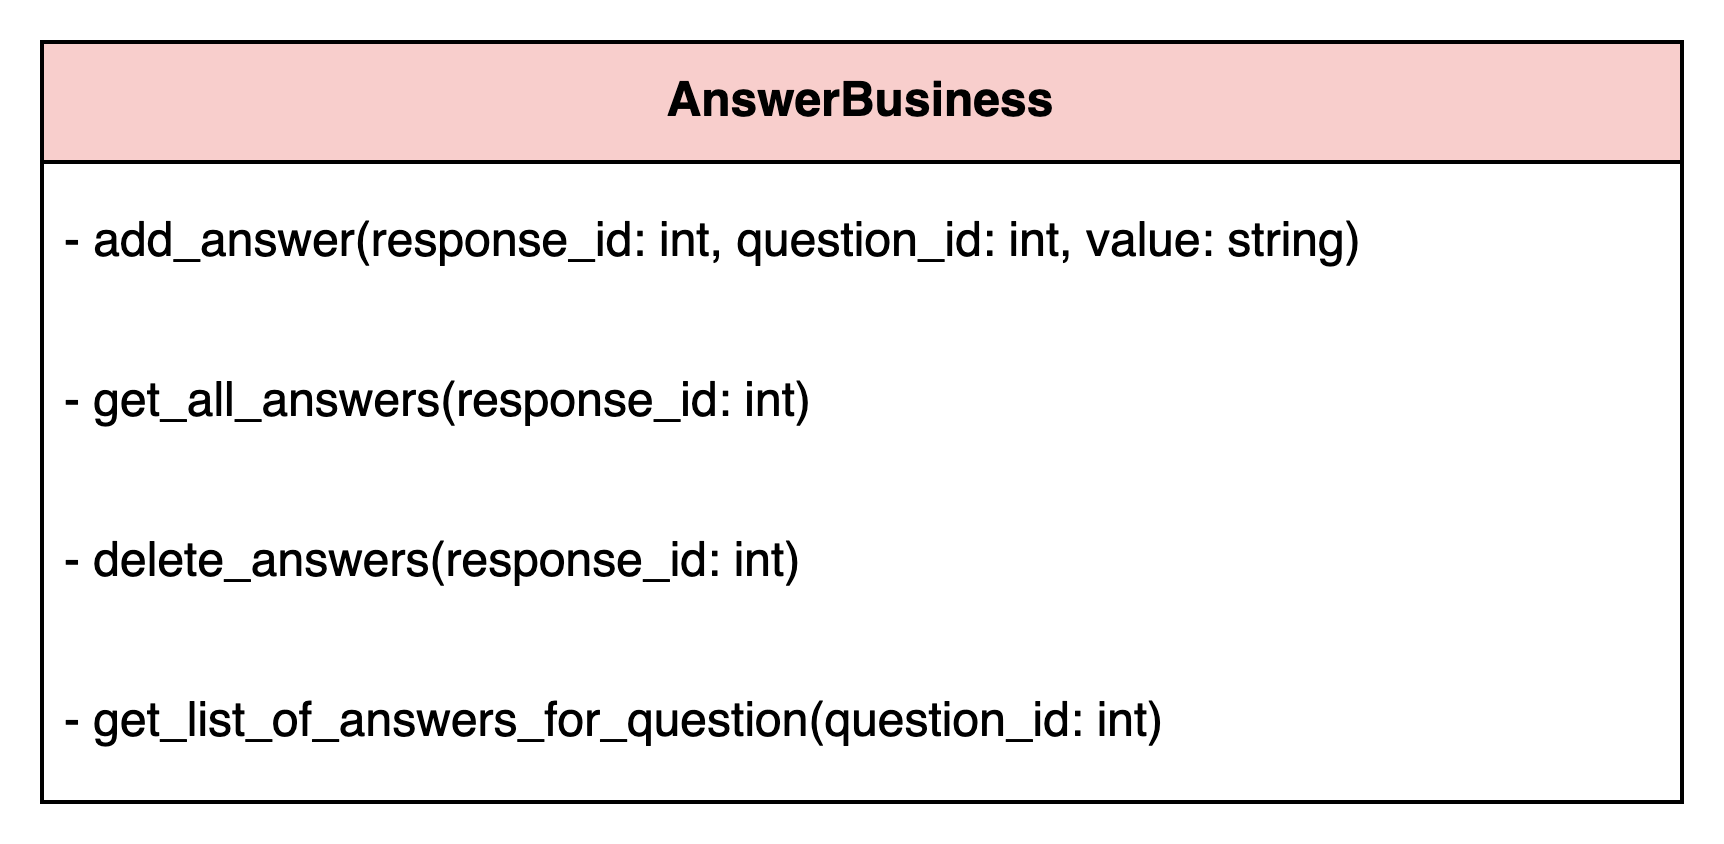
\includegraphics[ width = 0.5\linewidth]{Content/Phân tích và thiết kế hệ thống/documents/Sơ đồ lớp/images/Business layer/answer.png}
    \vspace{0.5cm}
    \caption{Class AnswerBusiness trong Business layer}
    \label{fig:Class AnswerBusiness trong Business layer}
\end{figure}
\par
Class AnswerBusiness gồm những phương thức xử lý logic liên quan đến những câu trả lời của người dùng tương ứng với các câu hỏi trong bảng khảo sát. 
Một số phương thức xử lý chẳng hạn như lấy toàn bộ các câu trả lời, xóa câu trả lời,...
\begin{figure}[H]
    \centering
    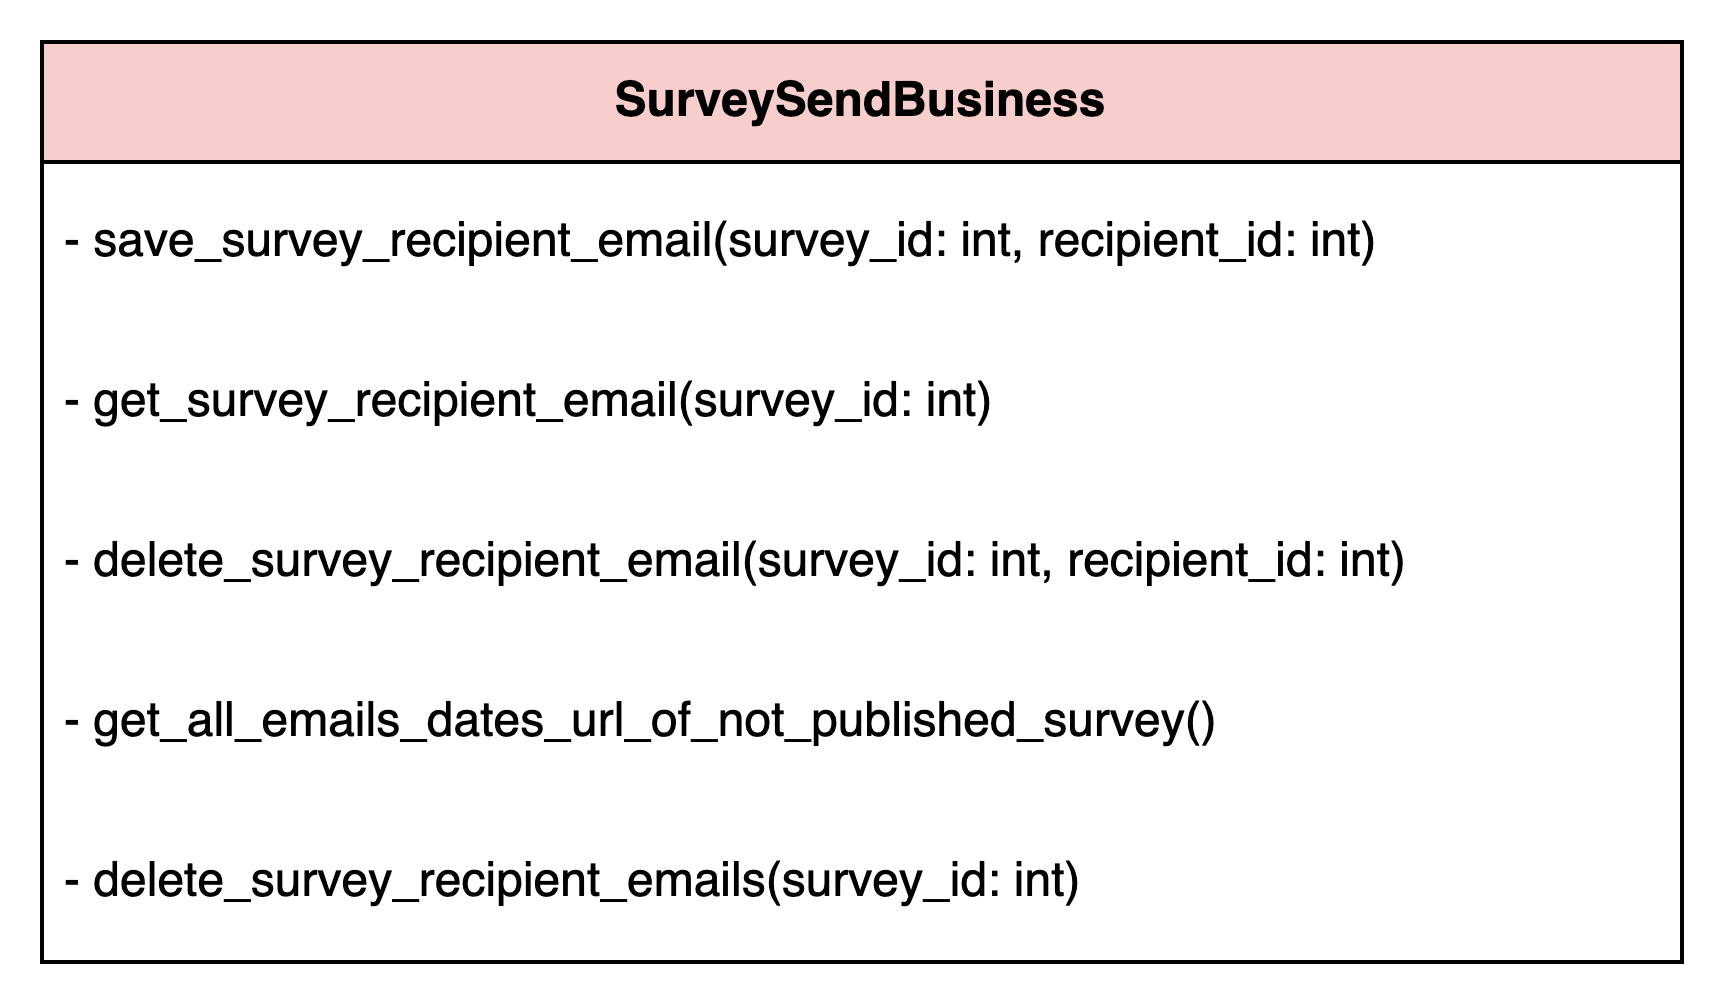
\includegraphics[ width = 0.5\linewidth]{Content/Phân tích và thiết kế hệ thống/documents/Sơ đồ lớp/images/Business layer/surveySend.png}
    \vspace{0.5cm}
    \caption{Class SurveySendBusiness trong Business layer}
    \label{fig:Class SurveySendBusiness trong Business layer}
\end{figure}
\par
Class SurveySendBusiness sẽ quản lý những logic xử lý về việc gửi bài khảo sát tới những người dùng cụ thể, và một số phương thức để phục 
vụ cho việc kiểm tra bài khảo sát đã được công bố hay chưa (tính năng tự động công bố hoặc đóng survey theo thời gian đã thiết lập).
\begin{figure}[H]
    \centering
    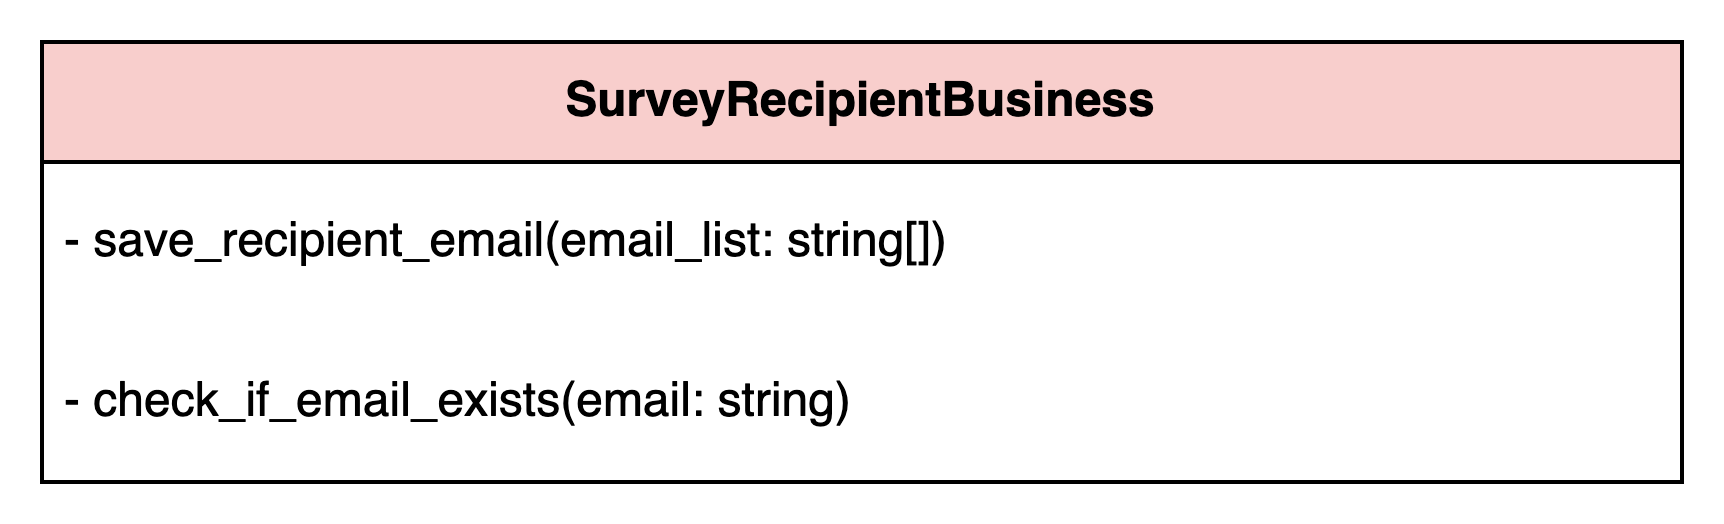
\includegraphics[ width = 0.5\linewidth]{Content/Phân tích và thiết kế hệ thống/documents/Sơ đồ lớp/images/Business layer/surveyRecipient.png}
    \vspace{0.5cm}
    \caption{Class SurveyRecipientBusiness trong Business layer}
    \label{fig:Class SurveyRecipientBusiness trong Business layer}
\end{figure}
\par
Class SurveyRecipientBusiness dùng để quản lý các logic liên quan đến những người dùng sẽ nhận email bài khảo sát được gửi từ hệ thống. 
Một số phương thức xử lý như lưu lại tạm thời email của người nhận, kiểm tra xem email đã tồn tại hay chưa.
\begin{figure}[H]
    \centering
    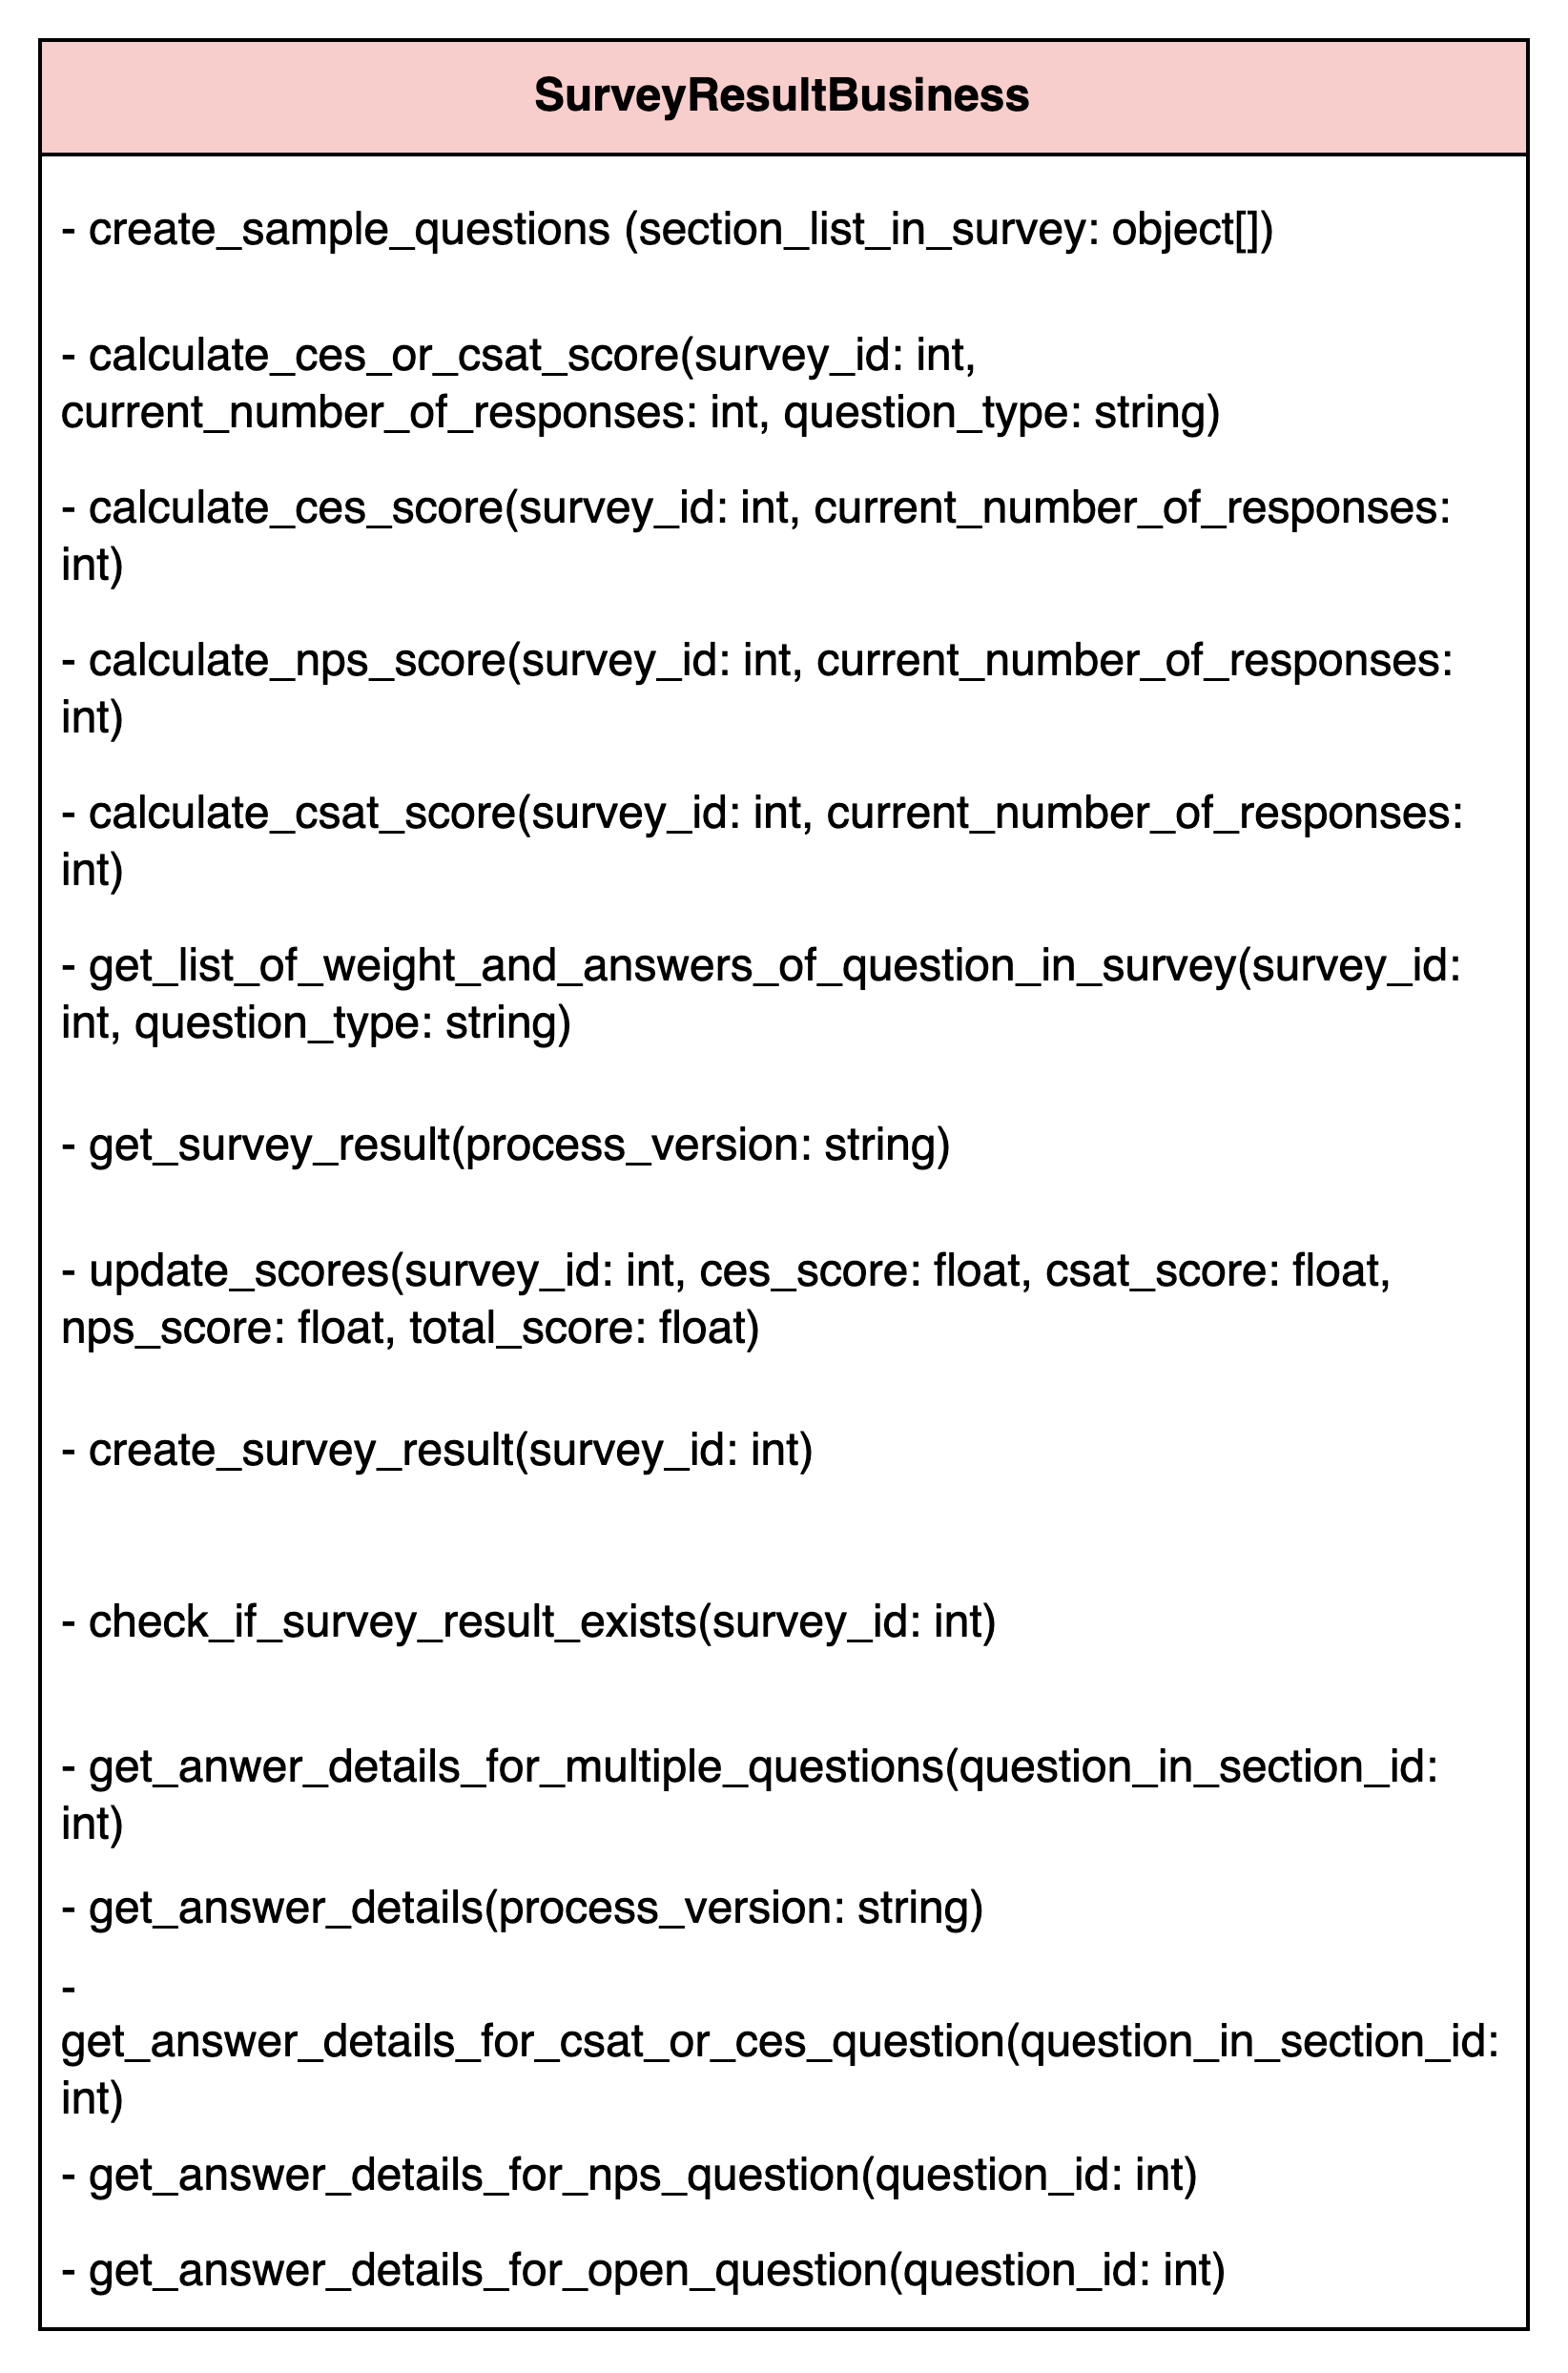
\includegraphics[ width = 0.5\linewidth]{Content/Phân tích và thiết kế hệ thống/documents/Sơ đồ lớp/images/Business layer/surveyResult.png}
    \vspace{0.5cm}
    \caption{Class SurveyResultBusiness trong Business layer}
    \label{fig:Class SurveyResultBusiness trong Business layer}
\end{figure}
\par
Class SurveyResultBusiness gồm những logic xử lý liên quan đến kết quả của bài khảo sát, chẳng hạn như tính toán các độ đo, điểm tổng thể của bài khảo sát, l
ấy thông tin chi tiết về việc trả lời mỗi câu hỏi của người dùng,...
\begin{figure}[H]
    \centering
    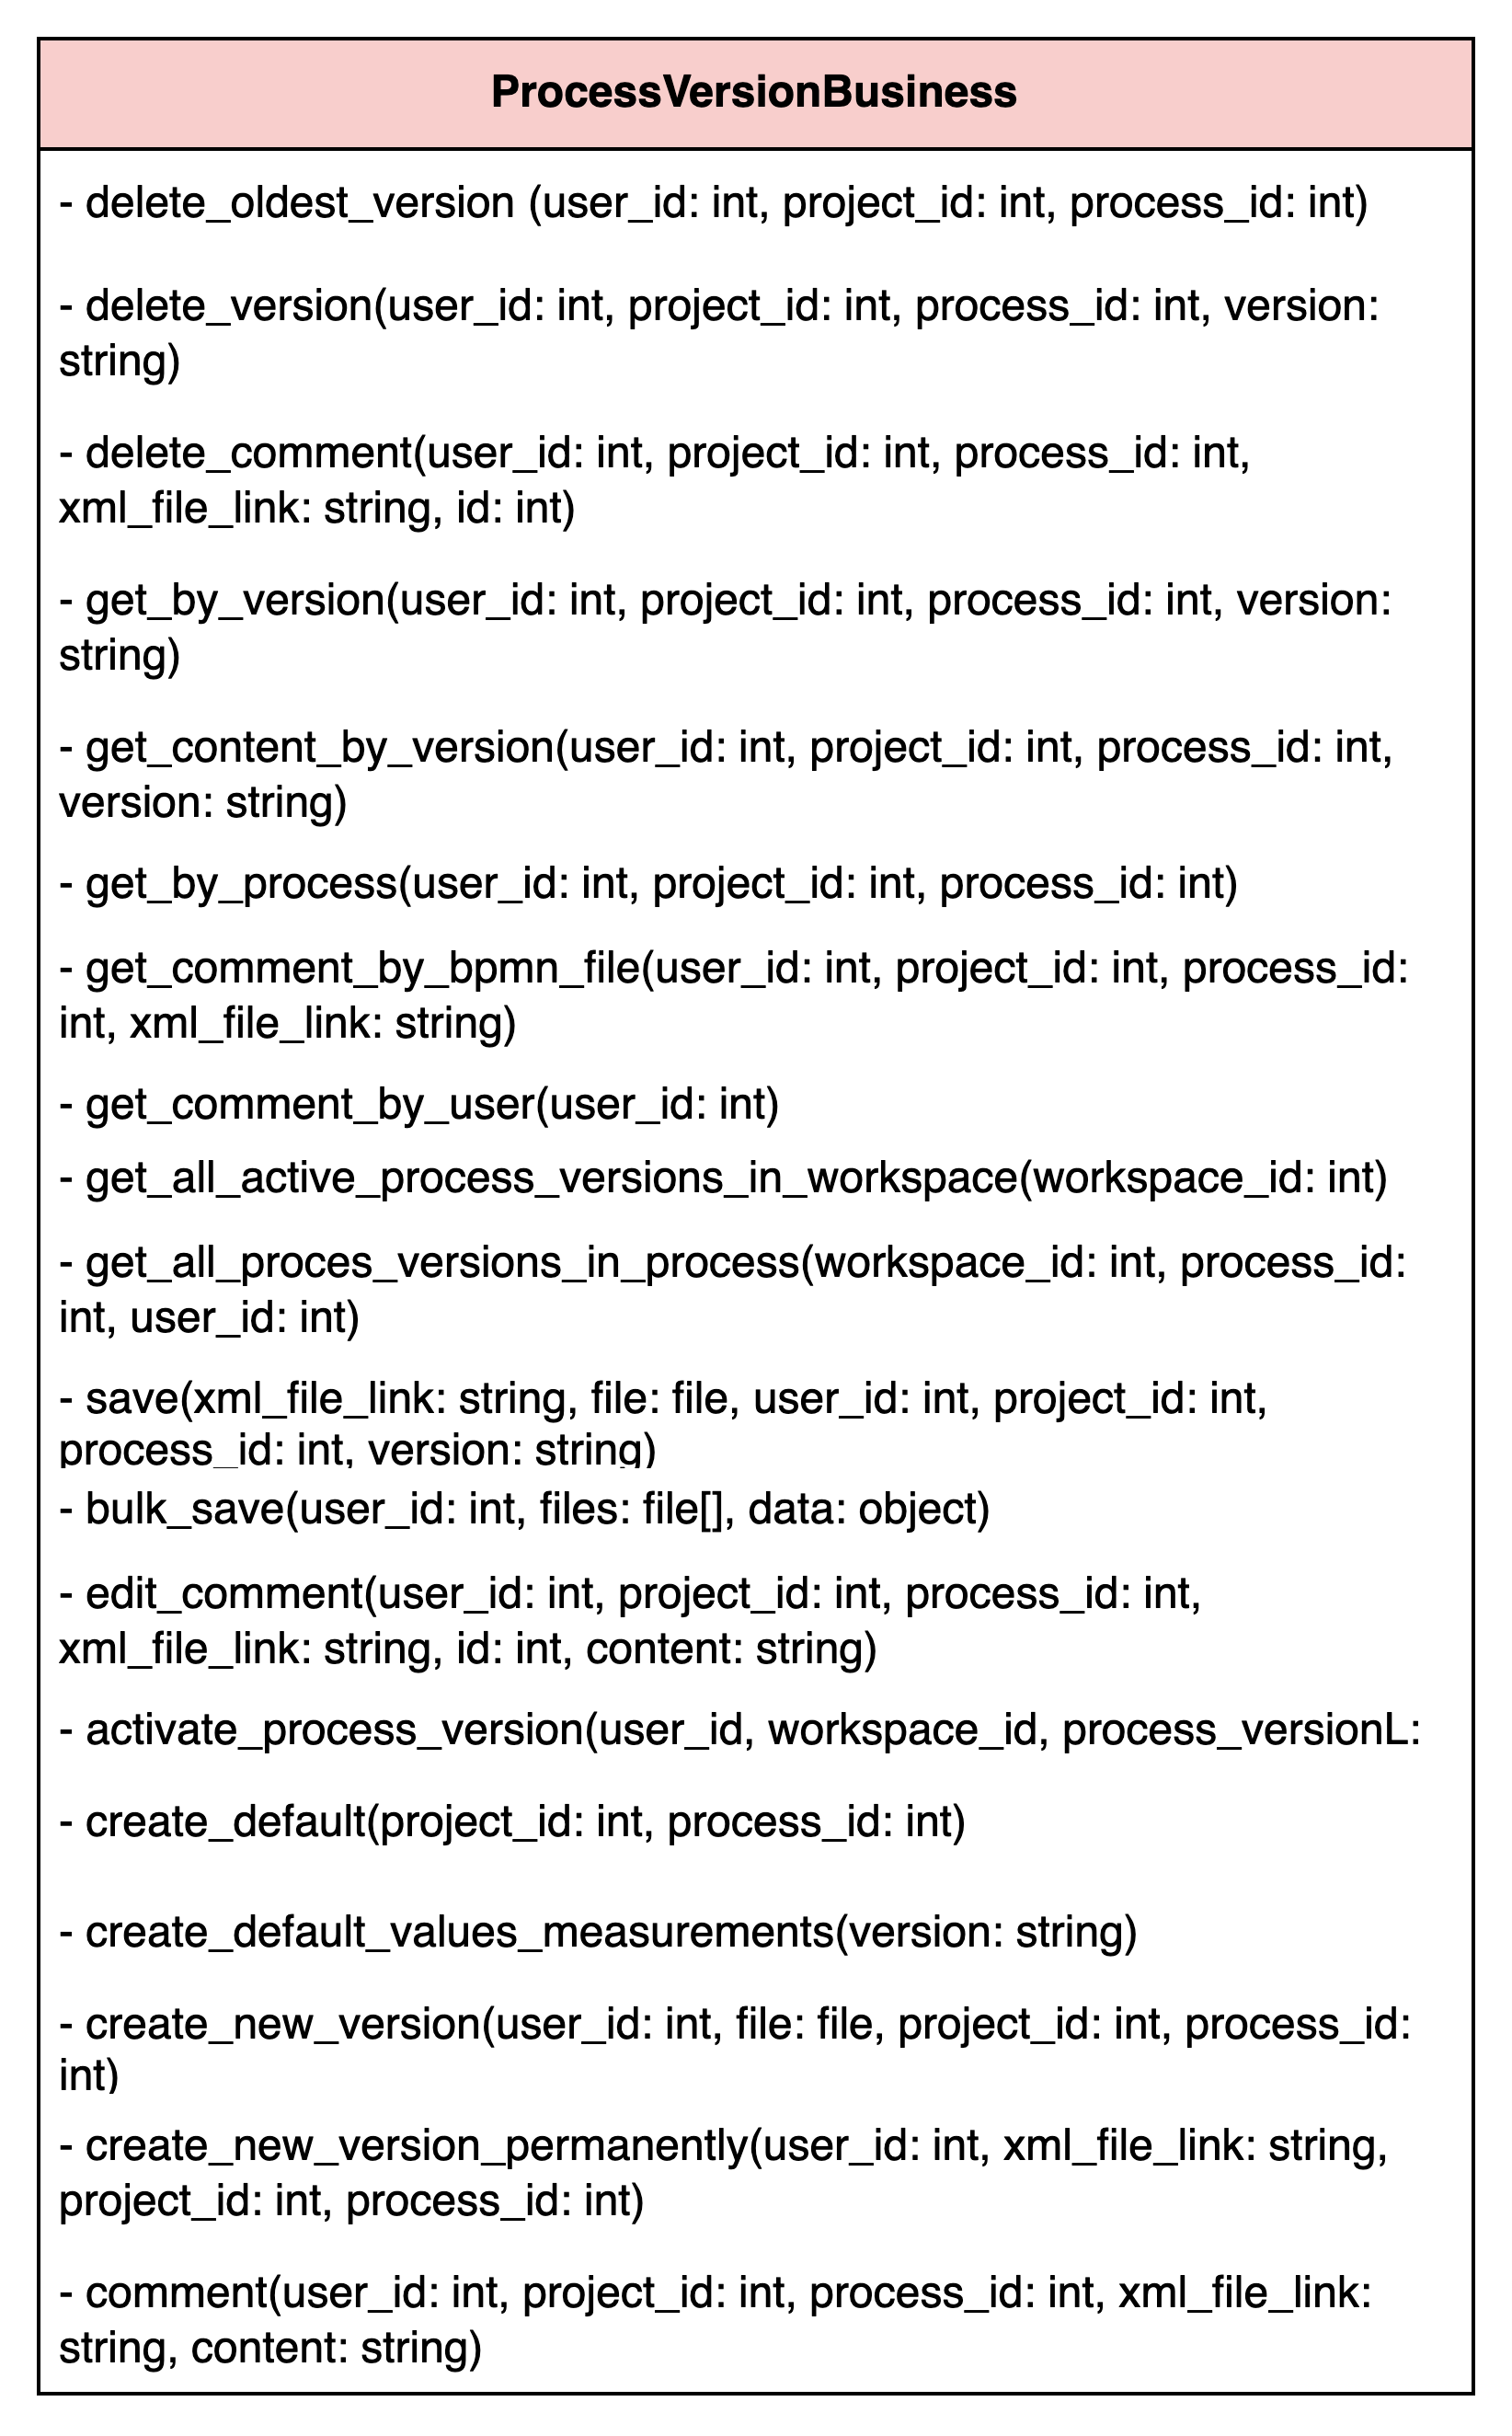
\includegraphics[ width = 0.5\linewidth]{Content/Phân tích và thiết kế hệ thống/documents/Sơ đồ lớp/images/Business layer/processVersion.png}
    \vspace{0.5cm}
    \caption{Class ProcessVersionBusiness trong Business layer}
    \label{fig:Class ProcessVersionBusiness trong Business layer}
\end{figure}
\par
Class ProcessVersionBusiness thừa kế lại những logic xử lý liên quan đến phiên bản của quy trình nghiệp vụ của đề tài trước đó, và 
phát triển thêm các hàm xử lý khác phục vụ cho đề tài này, chẳng hạn như kích hoạt các phiên bản và thay đổi phiên bản được kích hoạt nhằm 
phục vụ cho quá trinh khởi tạo process portfolio cho toàn bộ quy trình nghiệp vụ có trong Workspace.
\begin{figure}[H]
    \centering
    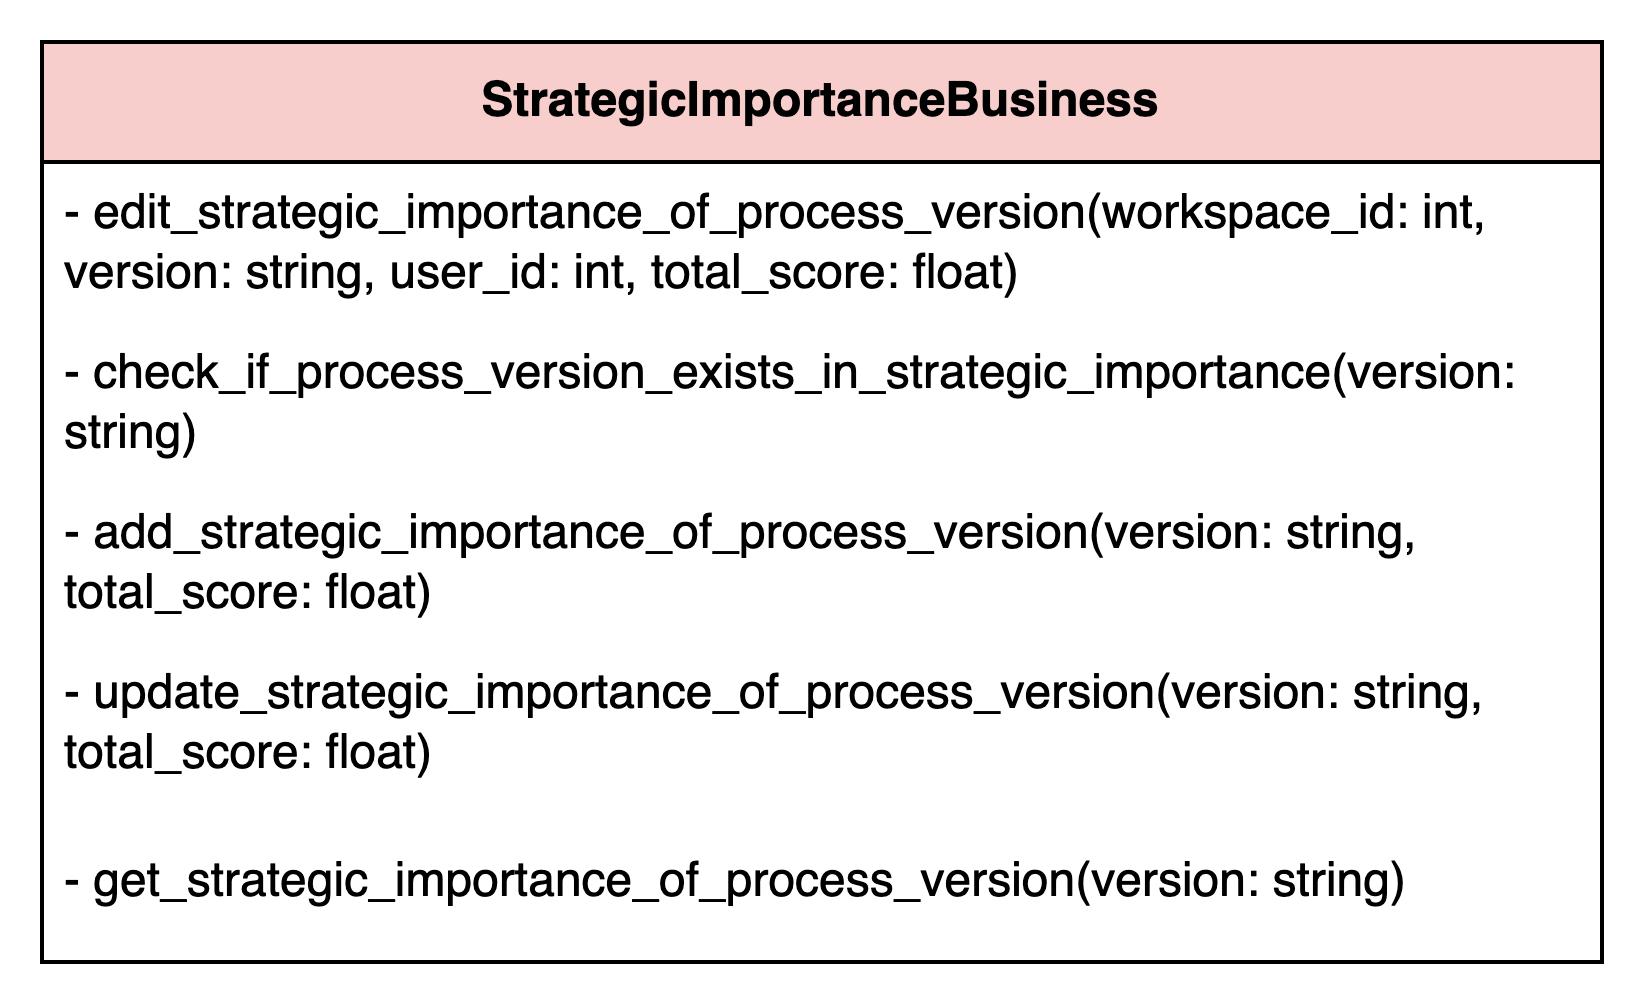
\includegraphics[ width = 0.5\linewidth]{Content/Phân tích và thiết kế hệ thống/documents/Sơ đồ lớp/images/Business layer/strategicImportance.png}
    \vspace{0.5cm}
    \caption{Class StrategicImportanceBusiness trong Business layer}
    \label{fig:Class StrategicImportanceBusiness trong Business layer}
\end{figure}
\par
Class StrategicImportanceBusiness quản lý logic liên quan đến độ đo độ quan trọng chiến lược của quy trình nghiệp vụ, 
chẳng hạn như cập nhật thay đổi của độ đo, lấy thông tin của độ đo để phục vụ việc hiển thị process portfolio của toàn bộ Workspace.
\begin{figure}[H]
    \centering
    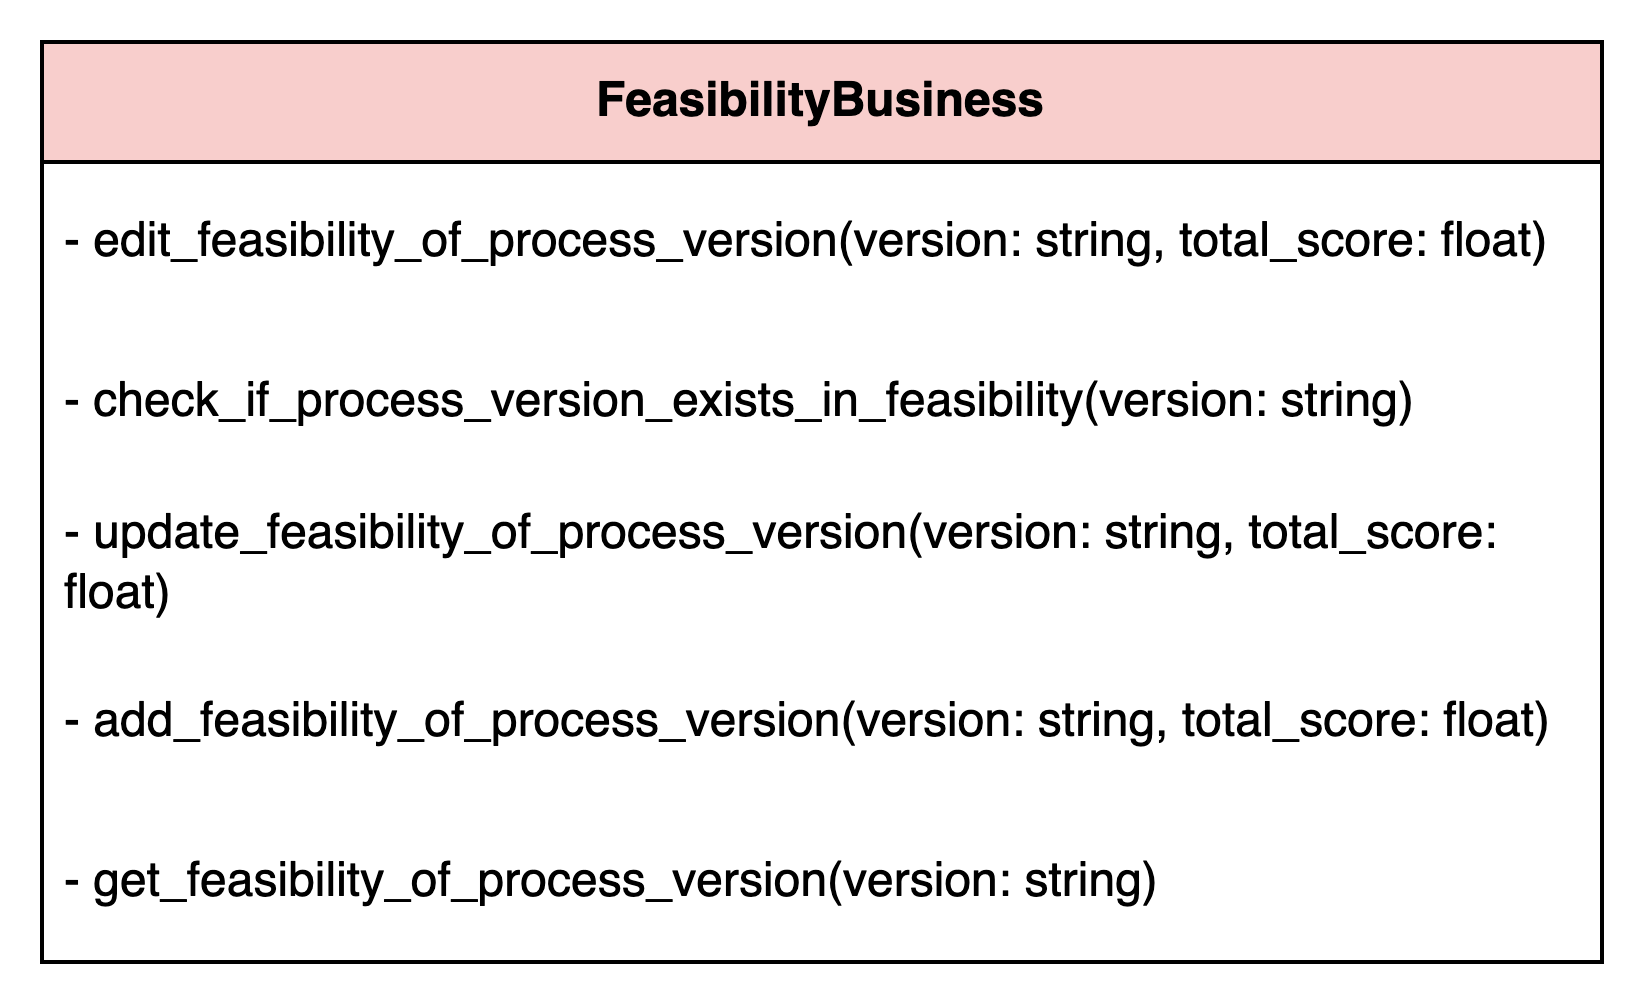
\includegraphics[ width = 0.5\linewidth]{Content/Phân tích và thiết kế hệ thống/documents/Sơ đồ lớp/images/Business layer/feasibility.png}
    \vspace{0.5cm}
    \caption{Class FeasibilityBusiness trong Business layer}
    \label{fig:Class FeasibilityBusiness trong Business layer}
\end{figure}
\par
Class FeasiblityBusiness quản lý logic liên quan đến độ đo tính khả thi của quy trình nghiệp vụ, chẳng hạn như thay đổi giá trị 
của tính khả thi và lấy thông tin chi tiết về độ đo này.
\begin{figure}[H]
    \centering
    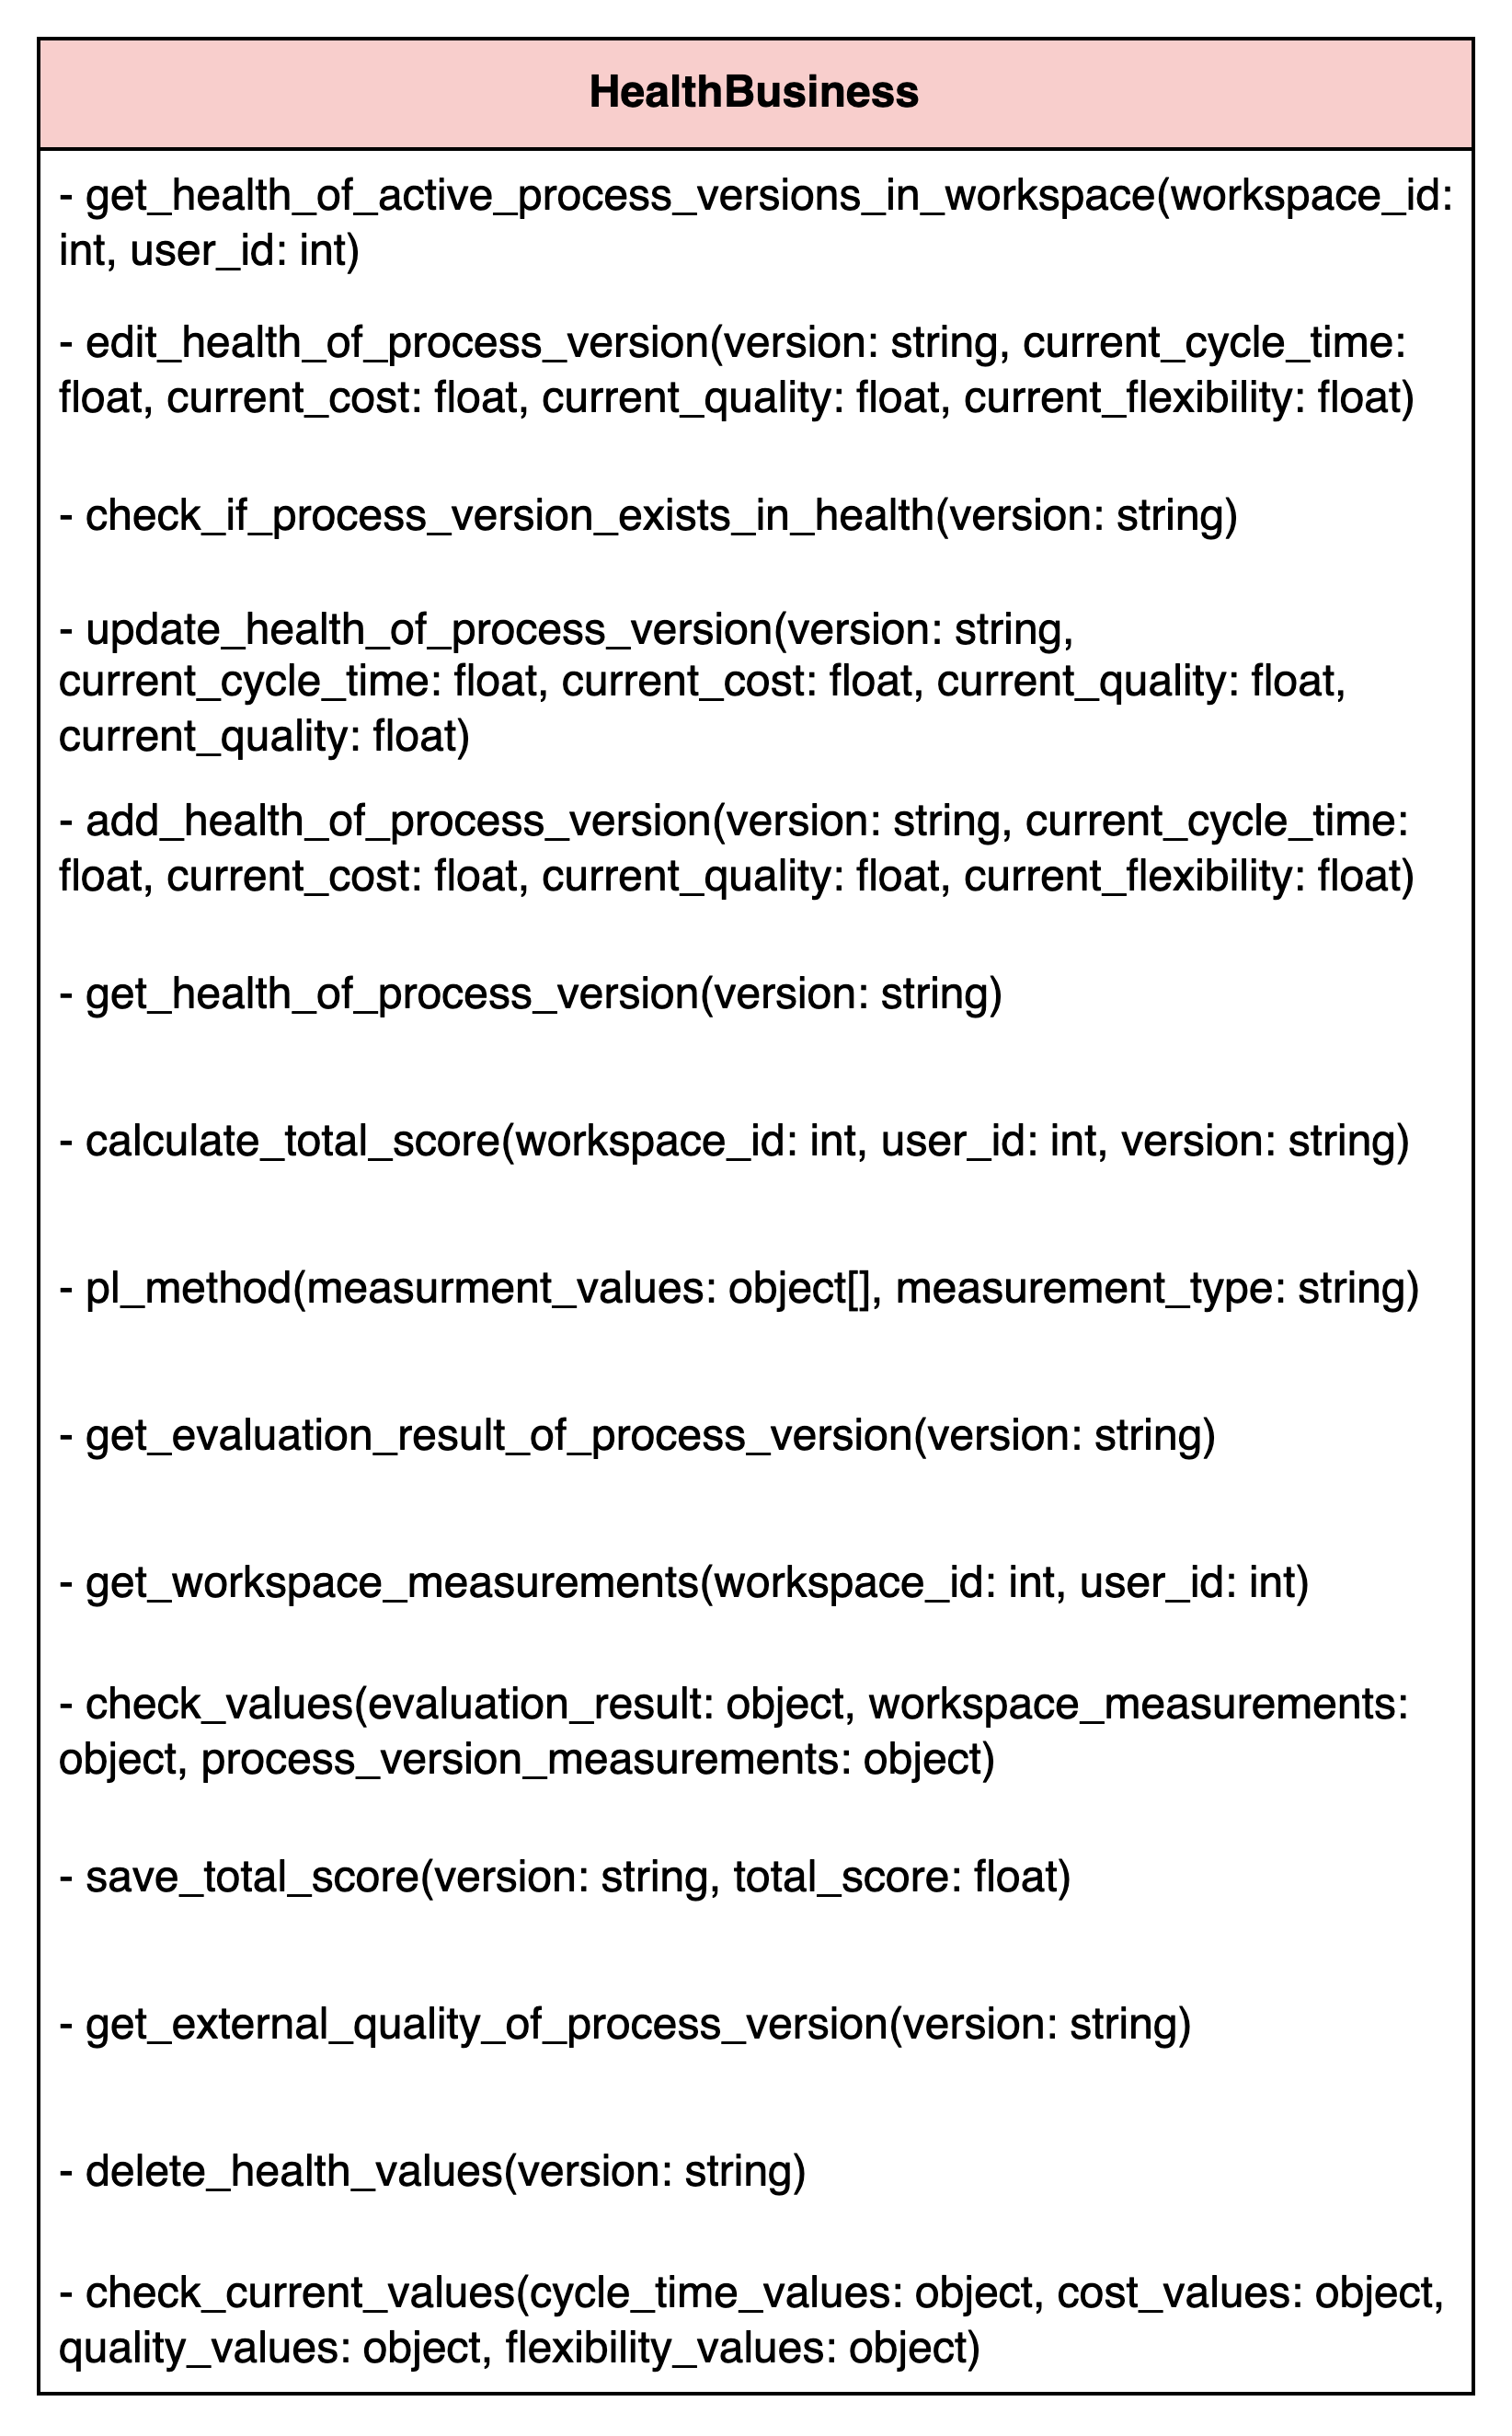
\includegraphics[ width = 0.5\linewidth]{Content/Phân tích và thiết kế hệ thống/documents/Sơ đồ lớp/images/Business layer/health.png}
    \vspace{0.5cm}
    \caption{Class HealthBusiness trong Business layer}
    \label{fig:Class HealthBusiness trong Business layer}
\end{figure}
\par
Class HealthBusiness bao gồm những logic xử lý về độ đo sức khỏe của quy trình nghiệp vụ, bao gồm những hàm xử lý như tính toán 
giá trị của độ đo này, lấy những tham số liên quan để tính toán được giá trị cuối cùng của độ đo,...
